\documentclass[
  man,
  longtable,
  nolmodern,
  notxfonts,
  notimes,
  colorlinks=true,linkcolor=blue,citecolor=blue,urlcolor=blue]{apa7}

\usepackage{amsmath}
\usepackage{amssymb}




\RequirePackage{longtable}
\RequirePackage{threeparttablex}

\makeatletter
\renewcommand{\paragraph}{\@startsection{paragraph}{4}{\parindent}%
	{0\baselineskip \@plus 0.2ex \@minus 0.2ex}%
	{-.5em}%
	{\normalfont\normalsize\bfseries\typesectitle}}

\renewcommand{\subparagraph}[1]{\@startsection{subparagraph}{5}{0.5em}%
	{0\baselineskip \@plus 0.2ex \@minus 0.2ex}%
	{-\z@\relax}%
	{\normalfont\normalsize\bfseries\itshape\hspace{\parindent}{#1}\textit{\addperi}}{\relax}}
\makeatother




\usepackage{longtable, booktabs, multirow, multicol, colortbl, hhline, caption, array, float, xpatch}
\usepackage{subcaption}


\renewcommand\thesubfigure{\Alph{subfigure}}
\setcounter{topnumber}{2}
\setcounter{bottomnumber}{2}
\setcounter{totalnumber}{4}
\renewcommand{\topfraction}{0.85}
\renewcommand{\bottomfraction}{0.85}
\renewcommand{\textfraction}{0.15}
\renewcommand{\floatpagefraction}{0.7}

\usepackage{tcolorbox}
\tcbuselibrary{listings,theorems, breakable, skins}
\usepackage{fontawesome5}

\definecolor{quarto-callout-color}{HTML}{909090}
\definecolor{quarto-callout-note-color}{HTML}{0758E5}
\definecolor{quarto-callout-important-color}{HTML}{CC1914}
\definecolor{quarto-callout-warning-color}{HTML}{EB9113}
\definecolor{quarto-callout-tip-color}{HTML}{00A047}
\definecolor{quarto-callout-caution-color}{HTML}{FC5300}
\definecolor{quarto-callout-color-frame}{HTML}{ACACAC}
\definecolor{quarto-callout-note-color-frame}{HTML}{4582EC}
\definecolor{quarto-callout-important-color-frame}{HTML}{D9534F}
\definecolor{quarto-callout-warning-color-frame}{HTML}{F0AD4E}
\definecolor{quarto-callout-tip-color-frame}{HTML}{02B875}
\definecolor{quarto-callout-caution-color-frame}{HTML}{FD7E14}

%\newlength\Oldarrayrulewidth
%\newlength\Oldtabcolsep


\usepackage{hyperref}




\providecommand{\tightlist}{%
  \setlength{\itemsep}{0pt}\setlength{\parskip}{0pt}}
\usepackage{longtable,booktabs,array}
\usepackage{calc} % for calculating minipage widths
% Correct order of tables after \paragraph or \subparagraph
\usepackage{etoolbox}
\makeatletter
\patchcmd\longtable{\par}{\if@noskipsec\mbox{}\fi\par}{}{}
\makeatother
% Allow footnotes in longtable head/foot
\IfFileExists{footnotehyper.sty}{\usepackage{footnotehyper}}{\usepackage{footnote}}
\makesavenoteenv{longtable}

\usepackage{graphicx}
\makeatletter
\newsavebox\pandoc@box
\newcommand*\pandocbounded[1]{% scales image to fit in text height/width
  \sbox\pandoc@box{#1}%
  \Gscale@div\@tempa{\textheight}{\dimexpr\ht\pandoc@box+\dp\pandoc@box\relax}%
  \Gscale@div\@tempb{\linewidth}{\wd\pandoc@box}%
  \ifdim\@tempb\p@<\@tempa\p@\let\@tempa\@tempb\fi% select the smaller of both
  \ifdim\@tempa\p@<\p@\scalebox{\@tempa}{\usebox\pandoc@box}%
  \else\usebox{\pandoc@box}%
  \fi%
}
% Set default figure placement to htbp
\def\fps@figure{htbp}
\makeatother


% definitions for citeproc citations
\NewDocumentCommand\citeproctext{}{}
\NewDocumentCommand\citeproc{mm}{%
  \begingroup\def\citeproctext{#2}\cite{#1}\endgroup}
\makeatletter
 % allow citations to break across lines
 \let\@cite@ofmt\@firstofone
 % avoid brackets around text for \cite:
 \def\@biblabel#1{}
 \def\@cite#1#2{{#1\if@tempswa , #2\fi}}
\makeatother
\newlength{\cslhangindent}
\setlength{\cslhangindent}{1.5em}
\newlength{\csllabelwidth}
\setlength{\csllabelwidth}{3em}
\newenvironment{CSLReferences}[2] % #1 hanging-indent, #2 entry-spacing
 {\begin{list}{}{%
  \setlength{\itemindent}{0pt}
  \setlength{\leftmargin}{0pt}
  \setlength{\parsep}{0pt}
  % turn on hanging indent if param 1 is 1
  \ifodd #1
   \setlength{\leftmargin}{\cslhangindent}
   \setlength{\itemindent}{-1\cslhangindent}
  \fi
  % set entry spacing
  \setlength{\itemsep}{#2\baselineskip}}}
 {\end{list}}
\usepackage{calc}
\newcommand{\CSLBlock}[1]{\hfill\break\parbox[t]{\linewidth}{\strut\ignorespaces#1\strut}}
\newcommand{\CSLLeftMargin}[1]{\parbox[t]{\csllabelwidth}{\strut#1\strut}}
\newcommand{\CSLRightInline}[1]{\parbox[t]{\linewidth - \csllabelwidth}{\strut#1\strut}}
\newcommand{\CSLIndent}[1]{\hspace{\cslhangindent}#1}





\usepackage{newtx}

\defaultfontfeatures{Scale=MatchLowercase}
\defaultfontfeatures[\rmfamily]{Ligatures=TeX,Scale=1}





\title{Latent Variable Moderated Mediation Using Correct and
Misspecified Models}


\shorttitle{Moderated Mediation With Latent Variables}


\usepackage{etoolbox}








\authorsnames{Felipe Fontana Vieira,Yves Rosseel}





\affiliation{
{Department of Data Analysis, Faculty of Psychology and Educational
Sciences, Ghent University}}




\leftheader{Vieira and Rosseel}



\abstract{Moderated mediation is seldom estimated with latent variables,
and its estimation methods have rarely been compared under
misspecification. In a preregistered simulation we evaluated three
estimation approaches of a latent moderated mediation model, the local
structural-after-measurement approach (LSAM) and two system-wide
methods, across sample size, interaction magnitude, reliability,
predictor distribution, and nine (mis)specification conditions. Under
correct specification, all recovered the interaction coefficient and
index of moderated mediation, differing modestly in bias, root mean
square error, coverage, standard errors, Type I error, and power. Under
misspecification, LSAM was most robust, leaving some estimates
unaffected by omissions that biased the system-wide approaches, although
most misspecifications degraded performance. }

\keywords{moderated mediation, structural equation modeling, latent
interaction, measurement error, model misspecification}

\authornote{\par{\addORCIDlink{Felipe Fontana
Vieira}{0009-0006-0949-6569}}\par{\addORCIDlink{Yves
Rosseel}{0000-0002-4129-4477}} 
\par{ }
\par{This study was preregistered. The preregistration, data, code, and
materials for this manuscript can be found at
\url{https://doi.org/10.5281/zenodo.20703258}.  The authors report there
are no competing interests to declare. Generative AI (Claude, Anthropic)
was used to assist with language editing and for creating the figures.
All content was reviewed and approved by the authors. This project was
funded by the Special Research Fund (BOF) of Ghent University
(BOF/24J/2023/144). We gratefully acknowledge the Borchard Foundation
for supporting the work summarized in this article. We also thank Sofia
Morelli for the helpful comments and discussions.  Author roles were
classified using the Contributor Role Taxonomy (CRediT;
https://credit.niso.org/) as follows:  Felipe Fontana
Vieira:   Conceptualization, Methodology, Software, Investigation, Data
curation, Formal analysis, Visualization, Writing - original
draft, Writing - review \& editing; Yves
Rosseel:   Conceptualization, Methodology, Software, Supervision, Writing
- review \& editing, Funding acquisition}
\par{Correspondence concerning this article should be addressed
to Felipe Fontana Vieira, Department of Data Analysis, Faculty of
Psychology and Educational Sciences, Ghent University, Henri Dunantlaan
2, Ghent 9000, Belgium, Email: \href{mailto:felipe.fontanavieira@ugent.be}{felipe.fontanavieira@ugent.be}}
}

\makeatletter
\let\endoldlt\endlongtable
\def\endlongtable{
\hline
\endoldlt
}
\makeatother
\RequirePackage{longtable}
\DeclareDelayedFloatFlavor{longtable}{table}

\urlstyle{same}



\raggedbottom
\usepackage{pdflscape}
\makeatletter
\@ifpackageloaded{caption}{}{\usepackage{caption}}
\AtBeginDocument{%
\ifdefined\contentsname
  \renewcommand*\contentsname{Table of contents}
\else
  \newcommand\contentsname{Table of contents}
\fi
\ifdefined\listfigurename
  \renewcommand*\listfigurename{List of Figures}
\else
  \newcommand\listfigurename{List of Figures}
\fi
\ifdefined\listtablename
  \renewcommand*\listtablename{List of Tables}
\else
  \newcommand\listtablename{List of Tables}
\fi
\ifdefined\figurename
  \renewcommand*\figurename{Figure}
\else
  \newcommand\figurename{Figure}
\fi
\ifdefined\tablename
  \renewcommand*\tablename{Table}
\else
  \newcommand\tablename{Table}
\fi
}
\@ifpackageloaded{float}{}{\usepackage{float}}
\floatstyle{ruled}
\@ifundefined{c@chapter}{\newfloat{codelisting}{h}{lop}}{\newfloat{codelisting}{h}{lop}[chapter]}
\floatname{codelisting}{Listing}
\newcommand*\listoflistings{\listof{codelisting}{List of Listings}}
\makeatother
\makeatletter
\makeatother
\makeatletter
\@ifpackageloaded{caption}{}{\usepackage{caption}}
\@ifpackageloaded{subcaption}{}{\usepackage{subcaption}}
\makeatother

% From https://tex.stackexchange.com/a/645996/211326
%%% apa7 doesn't want to add appendix section titles in the toc
%%% let's make it do it
\makeatletter
\xpatchcmd{\appendix}
  {\par}
  {\addcontentsline{toc}{section}{\@currentlabelname}\par}
  {}{}
\makeatother

%% Disable longtable counter
%% https://tex.stackexchange.com/a/248395/211326

\usepackage{etoolbox}

\makeatletter
\patchcmd{\LT@caption}
  {\bgroup}
  {\bgroup\global\LTpatch@captiontrue}
  {}{}
\patchcmd{\longtable}
  {\par}
  {\par\global\LTpatch@captionfalse}
  {}{}
\apptocmd{\endlongtable}
  {\ifLTpatch@caption\else\addtocounter{table}{-1}\fi}
  {}{}
\newif\ifLTpatch@caption
\makeatother

\begin{document}

\maketitle




\setlength\LTleft{0pt}




Mediation analysis is a well-known procedure in the behavioral and
social sciences (Charlton et al., 2021; Hayes, 2018; Pieters, 2017;
Preacher et al., 2007). In its basic and standard form, the effect of an
independent variable on an outcome is decomposed into a direct effect
and an indirect effect transmitted through a mediator, with all
variables observed. This single mediator model has since been extended
in a number of directions, most relevant here being the case in which
the indirect effect is allowed to depend on a moderator (Edwards \&
Lambert, 2007; Hayes, 2015; MacKinnon et al., 2007; Montoya, 2024;
Preacher et al., 2007).

In this context, a fundamental concern may arise from measurement. Many
constructs under investigation are not directly observed but are
measured indirectly through multiple items, that is, they are latent
variables (Bollen \& Hoyle, 2012). When such constructs are reduced to
summary scores (e.g., a sum or mean of the items) and analyzed as though
they were observed, a restrictive measurement structure is imposed
rather than tested (McNeish \& Wolf, 2020) and measurement error is left
unmodeled. This error can attenuate or inflate the indirect effect and
distort inferences about it (Cole \& Preacher, 2014; Hoyle \& Kenny,
1999), and it is especially consequential for the mediator, which acts
at once as a predictor and an outcome (Gonzalez \& MacKinnon, 2021). The
problem is compounded under moderation, where the product term is even
less reliable than either of its constituents (Bohrnstedt \& Marwell,
1978; Busemeyer \& Jones, 1983). To address this, structural equation
modeling (SEM) with latent variables has been advocated, especially in
the context of mediation (Cheung \& Lau, 2008; Falk \& Biesanz, 2015;
Ledgerwood \& Shrout, 2011; Montoya, 2024). It estimates structural
relationships between common factors, from which indicator-specific
unique variance has been partitioned, provided the measurement model is
correctly specified (Bollen, 1989; DeShon, 1998; Rhemtulla et al.,
2020). Yet we also note that latent variables do not necessarily improve
power in general, whether for interactions or not (Cham et al., 2012;
Ledgerwood \& Shrout, 2011; Wang \& Rhemtulla, 2021).

Moderated mediation with latent variables is not straightforward in
terms of statistical estimation. Indeed, a latent interaction\footnote{We
  use interaction and moderation interchangeably, as the focus is on
  estimation, but we highlight they imply different interpretations and
  causal assumptions (VanderWeele, 2009). An interaction also need not
  be a product term, although that is the most common functional form
  used by researchers (Rimpler et al., 2026).} involves the product of
two latent variables, which is unobserved and nonnormal even when its
constituents are normal (Kelava \& Brandt, 2022). Following this, a
number of methods have been proposed to estimate nonlinear effects among
latent variables (e.g., Boker et al., 2023; Bollen, 1995; Kenny \& Judd,
1984; Klein \& Moosbrugger, 2000; Klein \& Muthén, 2007; Marsh et al.,
2004; Mooijaart \& Bentler, 2010). Most adopt a joint (``system-wide'')
estimation strategy, in which the measurement and structural parameters
are estimated simultaneously. This is the case of the two best-known
methods, latent moderated structural equations (LMS) and the
unconstrained product indicator (UPI) approach. Opposed to these are
structural-after-measurement (SAM) approaches (Cox \& Kelcey, 2021;
Holst \& Budtz-Jørgensen, 2020; Ng \& Chan, 2020; Rosseel et al., 2025;
Wall \& Amemiya, 2000, 2003), in which the measurement model is
estimated first and the structural model afterward with the measurement
parameters held fixed. Many of these approaches have so far been rarely
applied in practice, likely held back by limited software, slow
estimation, and error-prone implementations. With recent open-source
implementations (Holst \& Budtz-Jørgensen, 2020; Rosseel et al., 2025;
Slupphaug et al., 2025) and non-commercial software (Keller, 2025), this
is likely to change.

Beyond estimation, a further consideration concerns interpretation.
Mediation is a hypothesis about causal effects, and causal
interpretation requires identification assumptions that \emph{may} not
be verified from the data alone (Imai et al., 2010; Morelli et al.,
2026; Rohrer et al., 2022). With latent variable models, further caution
is needed (Sterner et al., 2024; VanderWeele \& Vansteelandt, 2022). We
focus on one that is central to interpretation: the estimated latent
variables must validly represent the intended constructs (Gonzalez \&
MacKinnon, 2021). In fact, when they do not, the model is subject to
interpretational confounding (Burt, 1976), a discrepancy between the
empirical meaning assigned to a latent variable through its estimated
measurement parameters and the meaning intended by the researcher. This
reflects an underlying property of system-wide estimation, namely that
the consequences of a misspecification are not confined to the part of
the model in which it occurs (Bainter \& Bollen, 2014). Burt (1976)
proposed estimating the measurement model first, as a SAM approach does
(e.g., Rosseel \& Loh, 2024), so that the estimated latent variables and
their meaning do not depend on the structural model that follows,
although this does not imply that the structure is correct (VanderWeele
\& Vansteelandt, 2022).

To illustrate interpretational confounding, we specify a population
mediation model with three latent variables, X, M, and Y, each with
three indicators and all loadings equal to 1, and derive its
model-implied covariance matrix. We then set the covariances of the M
indicators with \(x_1\), \(x_2\), and \(x_3\) to 3, 1, and 1, rather
than the implied value of 2, so their association with M no longer
follows a single common factor. We fit the model to this matrix
(\(N = 200\)) with and without the mediator, by system-wide SEM and by
SAM, and compare the estimated loadings of \(x_2\) and \(x_3\). Without
the mediator, both approaches recover the true loadings of 1. Once the
mediator enters, the system-wide loadings drop to 0.41, whereas the SAM
loadings, estimated before the structural model, remain at 1.

Despite this, prior simulation work has examined latent interaction
estimation mainly under distributional misspecification (Brandt et al.,
2014; e.g., Cham et al., 2012; Lonati et al., 2025; Vieira et al.,
2026), and in only two cases under misspecification at the measurement
level (Brandt et al., 2020; Navarro \& Schermelleh-Engel, 2025), which
between them considered only the UPI and LMS among the approaches
studied here in limited settings. Moreover, when it comes to (moderated)
mediation, despite its popularity in applied research, only a few
studies have investigated it with latent variables, and those assumed a
correctly specified (and saturated) model (Cheung \& Lau, 2017; Falk \&
Biesanz, 2015; Feng et al., 2020). In this article, we therefore
evaluate three estimation approaches for a latent variable moderated
mediation model: local SAM (LSAM; Rosseel et al., 2025), LMS (Kelava et
al., 2011; Klein \& Moosbrugger, 2000), and UPI (Kelava \& Brandt, 2009;
Marsh et al., 2004). These approaches have been explained extensively in
previous research and we refer readers to it (e.g., Brandt et al., 2020;
Kelava et al., 2011; Lin et al., 2010; Lonati et al., 2025; Rosseel et
al., 2025; Slupphaug et al., 2025; Vieira et al., 2026).

\subsubsection{Present Research and
Contributions}\label{present-research-and-contributions}

This study makes two contributions. First, we evaluate LSAM alongside
LMS and UPI under both measurement and structural misspecification, in a
considerably broader design than previous studies, detailed in the next
section. The robustness of LSAM to model misspecification has itself
been examined only in linear models (Rosseel \& Loh, 2024), with later
research disputing it for measurement misspecifications and expecting it
to hold mainly for structural misspecifications in non-saturated
structural models (Robitzsch, 2022), a case not yet tested for models
with nonlinear effects. Second, we obtain inference for the index of
moderated mediation (imm; Hayes, 2015), a nonlinear function of the
structural parameters, with the Monte Carlo method (MacKinnon et al.,
2004; Preacher \& Selig, 2012) rather than the bootstrap used in the
latent variable studies above (Cheung \& Lau, 2017; Feng et al., 2020).
Bootstrapping is computationally expensive, and its variants differ
modestly in performance and rank differently depending on the criterion
(Falk \& Biesanz, 2015; Tibbe \& Montoya, 2022), whereas the Monte Carlo
method needs only the estimates and their covariance matrix. Whether it
performs adequately for the imm in the context under investigation,
which has not been examined, is a question we address here.

\section{Simulation Design and Performance
Evaluation}\label{simulation-design-and-performance-evaluation}

In this section we describe the design of the simulation study and the
measures used to evaluate performance, following the preregistration and
some recent recommendations for the conduct and reporting of simulation
studies (Pawel et al., 2026; Siepe et al., 2024).

\subsubsection{Population Model and
Estimands}\label{population-model-and-estimands}

We study a moderated mediation model among four latent variables: an
exogenous predictor \(X\), a moderator \(W\), a mediator \(M\), and an
outcome \(Y\). The structural model is as follows

\[
M = a_1 X + a_2 W + a_3\,(X \times W) + \zeta_M, \qquad
Y = b\,M + c'\,X + \zeta_Y.
\]

The primary estimands are the interaction coefficient (\(a_3\)) and the
imm (i.e., \(a_3 b\)). The remaining structural coefficients (\(a_1\),
\(a_2\), \(b\), \(c'\)) and the twelve freely estimated factor loadings
serve as secondary estimands. Note the imm is a derived quantity rather
than a free parameter, hence its true value is computed as \(a_3 b\)
implied by the correctly specified model.

Population values were fixed at \(a_1 = 0.4\), \(a_2 = 0.3\),
\(b = 0.5\), and \(c' = 0.15\), with \(\mathrm{cor}(X, W) = 0.3\). The
interaction coefficient \(a_3\) is a design factor (see below). These
coefficients, together with the structural disturbance variances, were
chosen so that under the baseline condition (normal exogenous predictors
and a correctly specified model) each dependent latent variable has
\(R^2 \approx 0.30\) at the interaction level \(a_3 = 0.20\). Also note
that, because \(a_3\) contributes to the variance of \(M\), the
explained variance is naturally higher with a larger \(a_3\) and lower
when its effect is null. Each latent variable is measured by four
congeneric indicators with loadings \(1.0\), \(0.8\), \(0.7\), and
\(0.6\). Figure~\ref{fig-model} shows the population model, where the
measurement and structural misspecifications studied below are drawn in
gray.

\begin{figure}[!htbp]

{\caption{{Population Model for the Simulation
Study.}{\label{fig-model}}}}

\begin{center}
\pandocbounded{\includegraphics[keepaspectratio]{article_files/figure-pdf/fig-model-1.pdf}}
\end{center}

\noindent \emph{Note.} \(X\),~\(W\), \(M\), and \(Y\) are latent
variables, each measured by four congeneric indicators. Circles are
latent variables and \(X{\times}W\) is the latent interaction. Black
elements form the correctly specified model that every approach fits
(\(a_1\), \(a_2\), \(a_3\), \(b\), \(c'\), and the \(X\)--\(W\)
covariance). Gray elements are the misspecifications present in the
population but omitted from the fitted model: two in the structural
part, an omitted moderator effect on the outcome (\(c_2\)) and an
omitted moderated direct effect (\(c_3\)); and two in the measurement
part, an omitted cross-loading of \(X\) on \(m_3\) (cl) and an omitted
residual covariance between \(m_3\) and \(y_3\) (rc). Residual variances
and intercepts are not shown.

\end{figure}

\subsubsection{Simulation Conditions}\label{simulation-conditions}

We employed a fully factorial design crossing five factors: sample size
(\(N \in \{100, 200, 300, 500\}\)), interaction magnitude
(\(a_3 \in \{0, 0.20, 0.40\}\)), measurement reliability (low \(= 0.5\),
high \(= 0.7\)), the distribution of the exogenous latent predictors
(normal, uniform, \(t_5\), and two \(\chi^2\) conditions with same- or
opposite-direction skewness), and the (mis)specification conditions
(nine cases; see Data Generation below). This yielded
\(4 \times 3 \times 2 \times 5 \times 9 = 1{,}080\) conditions, each
replicated 1,000 times.

Sample sizes cover the small to moderate range, where interaction terms
are estimated with limited power (Brandt et al., 2020; Lonati et al.,
2025). The interaction magnitudes include a null condition to assess
Type I error for the interaction coefficient and imm, and two nonzero
levels representing small and moderate latent moderation effects,
following previous research (Feng et al., 2020; Klein \& Moosbrugger,
2000). Reliability levels of \(0.5\) and \(0.7\) were chosen because
measurement error is amplified in product terms and is therefore
especially consequential for latent interaction estimation (Brandt et
al., 2020; Lonati et al., 2025; Vieira et al., 2026). Nonnormality of
the latent predictors is both empirically common and methodologically
central for latent interaction approaches, whose distributional
assumptions differ across approaches (Cham et al., 2012; Klein \&
Moosbrugger, 2000; Klein \& Muthén, 2007; Lonati et al., 2025; Vieira et
al., 2026). The misspecification conditions follow the moderated
mediation framework for the two structural omissions (Preacher et al.,
2007) and prior latent interaction simulation work for the two
measurement omissions (Brandt et al., 2020). They were also chosen as
interpretable violations, acting respectively as a measured
mediator--outcome confounder (Imai et al., 2010), a conflated moderated
direct effect (Edwards \& Lambert, 2007), exposure-correlated
measurement error in the mediator (Fritz et al., 2016; VanderWeele et
al., 2012), and a shared unmeasured cause of a mediator and an outcome
indicator (Cole et al., 2007). The misspecification cases are detailed
below.

\subsubsection{Estimation Approaches}\label{estimation-approaches}

We used LSAM (Rosseel et al., 2025; Rosseel \& Loh, 2024; Vieira et al.,
2026), with the measurement model estimated by maximum likelihood (ML)
in the first step and with standard errors obtained as in Vieira et al.
(2026) (see their Appendix A). In this case, the interacting predictors
\(X\) and \(W\) shared a single measurement block, while \(M\) and \(Y\)
formed their own blocks. We further used LMS (Klein \& Moosbrugger,
2000), with robust standard errors, and the extended UPI approach with
double mean centering (Kelava \& Brandt, 2009; Lin et al., 2010; Marsh
et al., 2004), estimated with robust ML, that is, with Huber--White
sandwich standard errors.

\subsubsection{Data Generation}\label{data-generation}

\hyperref[apx-calibration]{Appendix} describes the complete
data-generating mechanism in detail. Briefly, the latent variables \(X\)
and \(W\) were drawn from a bivariate distribution with
\(\operatorname{Cor}(X, W) = \rho = 0.3\), constructed with the
vine-to-anything (VITA) algorithm (Grønneberg et al., 2022). Five
exogenous distributions were examined, each standardized to mean \(0\)
and variance \(1\). Thus, the conditions differ only in distributional
shape, not in scale or location. Specifically, the normal condition
draws \(X, W \sim \mathcal{N}(0, 1)\) through a forced Gaussian copula,
whereas the remaining four combine nonnormal margins with a non-Gaussian
copula: uniform, \(t_5\), and two \(\chi^2(2)\) conditions in which
\(X\) and \(W\) are skewed in the same or in opposite directions. Then,
\(M\) and \(Y\) were generated from the structural equations above with
independent Gaussian disturbances
\(\zeta_M \sim \mathcal{N}(0, \psi_M)\) and
\(\zeta_Y \sim \mathcal{N}(0, \psi_Y)\), and the four indicators
(\(j = 1, \dots, 4\)) of each latent variable
\(\eta \in \{X, W, M, Y\}\) were formed as
\(z_{\eta j} = \lambda_j \eta + \delta_{\eta j}\), with loadings
\(\lambda = (1, 0.8, 0.7, 0.6)\) and Gaussian errors
\(\delta_{\eta j} \sim \mathcal{N}(0, \theta_{\eta j})\) whose variances
\(\theta_{\eta j}\) were scaled to the target reliability
\(\omega \in \{0.5, 0.7\}\).

The nine (mis)specification conditions comprise one correctly specified
condition and four types of misspecification, each at two empirically
calibrated magnitudes (standardized \(0.25\) and \(0.50\), detailed in
\hyperref[apx-calibration]{Appendix}), similar to Brandt et al. (2020).
Two are structural: an omitted direct effect of the moderator on the
outcome (\(c_2\)) and an omitted moderated direct effect (\(c_3\)). The
others are in the measurement model: a cross-loading of a mediator
indicator on \(X\) (\texttt{cl}) and a residual covariance between a
mediator and an outcome indicator (\texttt{rc}). In every case the
effect is present in the population but omitted from the estimated
model.

\subsubsection{Convergence, Outliers, and Inadmissible
Solutions}\label{convergence-outliers-and-inadmissible-solutions}

Following previous research (Lonati et al., 2025; Vieira et al., 2026),
replications were screened before analysis in two sequential steps. In
both, a replication that failed the screening for any one estimator was
removed for all three, so that every estimator is compared on an
identical set of replications. First, we checked convergence. A solution
was treated as nonconverged when any estimate, standard error, or
confidence-interval bound of any structural coefficient or loading was
missing or non-finite, and a replication was removed from all approaches
whenever any one of them did not converge. Second, among the remaining
replications, we screened for outliers, identified per condition,
method, and parameter of interest as point estimates more than three
interquartile ranges below the first or above the third quartile,
together with replications whose estimated standard error exceeded
\(10\) on any parameter of interest\footnote{We added the standard error
  criterion because some replications retained anomalous standard errors
  despite acceptable point estimates. It additionally removed 125
  replications (about \(0.01\%\) of the globally converged ones),
  predominantly for UPI at the smallest sample size with low reliability
  and skewed \(\chi^2\) predictors.}. Again, a replication identified as
an outlier for any estimation approach was removed from all of them. We
also identified inadmissible solutions, where any residual (unique)
variance was nonpositive or the covariance matrix of the exogenous
latent variables and latent disturbances was not positive definite.

\subsubsection{Performance Measures}\label{performance-measures}

Performance was assessed with the measures implemented in the
\emph{simhelpers} package (Joshi \& Pustejovsky, 2025), computed for the
imm, the structural coefficients, and the loadings. These measures, with
their empirical and Monte Carlo standard error (MCSE) calculations, are
listed in Table~\ref{tbl-performance}. Note that the MCSEs are obtained
in closed form where available and by jackknife otherwise. In addition,
where applicable, we report the rejection rate (Type I error when
\(a_3 = 0\), power otherwise).

\begin{table}

{\caption{{Subset of the Performance Measures for Evaluating Parameter
Estimates}{\label{tbl-performance}}}
\vspace{-20pt}}

\begin{center}

\begin{longtable*}{lll}
\toprule
Performance measure & Empirical calculation & MCSE\\
\midrule
\textit{Relative criteria} &  & \\
Relative bias & $\tfrac{\bar{\hat\theta}}{\theta}-1$ & $\sqrt{S_{\hat\theta}^2/(K\theta^2)}$\\
Relative RMSE & $\tfrac{1}{|\theta|}\sqrt{\tfrac{1}{K}\sum_{k=1}^{K}(\hat\theta_k-\theta)^2}$ & $\tfrac{1}{|\theta|}\sqrt{\tfrac{K-1}{K}\sum_{j=1}^{K}(\mathrm{RMSE}_{(j)}-\mathrm{RMSE})^2}$\\
\textit{Standard errors} &  & \\
Mean SE & $\overline{SE}=\tfrac{1}{K}\sum_{k=1}^{K}\widehat{SE}_k$ & ---\\
SE/SD ratio & $\overline{SE}/S_{\hat\theta}$ & ---\\
Relative bias of variance estimator & $\rho=\overline{SE^2}/S_{\hat\theta}^2$ & $\sqrt{\tfrac{K-1}{K}\sum_{j=1}^{K}(\rho_{(j)}-\rho)^2}$\\
\textit{Coverage} &  & \\
Coverage & $c=\tfrac{1}{K}\sum_{k=1}^{K}I(L_k\le\theta\le U_k)$ & $\sqrt{c(1-c)/K}$\\
\textit{Hypothesis testing} &  & \\
Rejection rate & $r=\tfrac{1}{K}\sum_{k=1}^{K}I(0\notin[L_k,U_k])$ & $\sqrt{r(1-r)/K}$\\
\bottomrule
\end{longtable*}
\end{center}

\vspace{-20pt}
\noindent \emph{Note.} \(\hat\theta_k\)~is the estimate of parameter
\(\theta\) in replication \(k\) (\(k = 1, \dots, K\) usable
replications), \(\bar{\hat\theta}\) its mean, \(S_{\hat\theta}^2\) its
sample variance, and \(S_{\hat\theta}\) its standard deviation (SD); the
root mean square error is
\(\mathrm{RMSE} = \sqrt{\tfrac{1}{K}\sum_k (\hat\theta_k-\theta)^2}\);
\(\widehat{SE}_k\) is the estimated standard error (SE),
\(\overline{SE^2} = \tfrac{1}{K}\sum_k \widehat{SE}_k^2\), and
\(L_k, U_k\) the confidence-interval limits; \(c\) and \(r\) denote
coverage and rejection rate, and \(\rho\) the relative bias of the
variance estimator. The subscript \((j)\) marks a leave-one-out
jackknife replicate. The MCSEs for relative RMSE and the relative bias
of the variance estimator are computed by jackknife; the others are
closed-form, and dashes mark MCSEs that are not computed.

\end{table}

Inference for the imm followed the Monte Carlo method as mentioned
before: for \(r = 1, \dots, R\) (with \(R = 20{,}000\)) we drew

\[
\bigl(a_3^{(r)}, b^{(r)}\bigr) \sim
\mathcal{N}_2\!\bigl((\hat a_3, \hat b),\, \hat\Sigma_{a_3 b}\bigr),
\qquad
\mathrm{imm}^{(r)} = a_3^{(r)}\, b^{(r)},
\]

where \(\hat\Sigma_{a_3 b}\) is the estimated covariance of
\((\hat a_3, \hat b)\), and took the \(2.5\)th and \(97.5\)th empirical
percentiles of \(\{\mathrm{imm}^{(r)}\}_{r=1}^{R}\) as the interval. The
structural coefficients and loadings use Wald-based intervals from the
same estimated covariance matrix of the parameter estimates.

\subsubsection{Reproducibility and Computational
Details}\label{reproducibility-and-computational-details}

All analyses were conducted in R (R Core Team, 2025) using the
\emph{lavaan} (Rosseel, 2012) and \emph{modsem} (Slupphaug et al., 2025)
packages for estimation, \emph{covsim} (Grønneberg et al., 2022) and
\emph{rvinecopulib} (Nagler \& Vatter, 2025) for data generation, and
\emph{simhelpers} (Joshi \& Pustejovsky, 2025) for performance
evaluation. Conditions were run in parallel with the \emph{parallel}
package. Reproducible and independent random-number streams across
workers were obtained with the L'Ecuyer-CMRG generator. The
computational environment was pinned with Nix (Dolstra et al., 2004) via
the \emph{rix} package (Rodrigues \& Baumann, 2026) to ensure
reproducibility, and the article was written with the \emph{apaquarto}
extension (Schneider, 2026). For the R version, package versions, code,
manuscript, and materials, see the project repository.

\section{Results}\label{results}

We present the results in three sections. First, the results for the
interaction coefficient and the imm are reported. We then turn to the
remaining structural coefficients (i.e., \(a_1\), \(a_2\), \(b\), and
\(c'\)), and we close with the estimated factor loadings, focusing
mainly on that of the cross-loaded indicator (\(m_3\)). Due to the large
number of conditions, we focus on a subset. In most figures we fix the
interaction coefficient at 0.2 and show \(N = 200\) and \(500\) for the
interaction coefficient and imm, and solely \(N = 500\) for the
structural coefficients and loadings. For the latter two, we further
restrict to high reliability, whereas the interaction coefficient and
imm are shown at both reliability levels. All results and detailed
convergence and outlier information are available in the repository.

\subsection{Convergence, Outliers, and Inadmissible
Solutions}\label{convergence-outliers-and-inadmissible-solutions-1}

Convergence was high throughout. LSAM converged in every replication
across all conditions, and LMS in at least \(99.9\%\). UPI was the least
stable, with its convergence rate falling to about \(92\%\) in the worst
condition (the smallest sample size, low reliability, and skewed
\(\chi^2\) predictors). At high reliability, however, UPI converged in
at least \(99\%\) of replications regardless of sample size,
distribution, or misspecification. Outliers were likewise rare, staying
below \(1\%\) in most conditions and reaching up to roughly \(11\%\) for
UPI and \(8\%\) for LSAM, only at \(N = 100\) with low reliability and
skewed (\(\chi^2\)) predictors. The results reported below did not
exclude inadmissible solutions, which arose almost exclusively for UPI;
excluding them leads to negligible changes, confined to the smallest
sample size, low reliability, \(\chi^2\) conditions.

\subsection{Main Structural Estimates}\label{main-structural-estimates}

\subsubsection{Relative Bias}\label{relative-bias}

We interpret values whose absolute relative bias exceeds 0.10 (10\%) as
biased, following previous research (Brandt et al., 2014; Vieira et al.,
2026). Under correct specification with normal predictors, all three
approaches recover both the interaction coefficient and imm without bias
at every sample size and reliability level, and the same holds under
uniform and \(t_5\) predictors apart from single LMS cells at
\(N = 100\) with low reliability (Figure~\ref{fig-baseline-bias-imm} and
Figure~\ref{fig-baseline-bias-a3}). Moreover, the \(\chi^2\) conditions
affect all three approaches, but differently. UPI and LSAM are biased
only at \(N = 100\) with low reliability, where UPI shows the largest
deviation, whereas LMS remains biased across all sample sizes at low
reliability, negatively under opposite skewness at the larger
interaction and positively under same skewness at the smaller one.

Under misspecification, \(c_2\) biases the imm for all three estimation
approaches across distributions, and so does \(c_3\) in most conditions,
as expected. The size of the bias nevertheless varies with the predictor
distribution, being largest under normal and same-skewness \(\chi^2\)
predictors and smallest under opposite-skewness \(\chi^2\) and \(t_5\)
predictors. For the interaction coefficient, \(c_2\) produces
essentially no bias for all approaches, whereas \(c_3\) leads to bias
under the system-wide approaches, mainly at low reliability. Among the
measurement omissions, \texttt{cl} leaves the imm unbiased except for
LMS in the \(\chi^2\) conditions, and attenuates the interaction
coefficient only under the system-wide methods. Last, \texttt{rc}
induces an upward bias in the imm at low reliability, most pronounced
for LMS under same-skewness \(\chi^2\), and leaves the interaction
coefficient largely unchanged. For the structural omissions, the bias
increases with the omission magnitude wherever present, and it is
generally larger at low reliability (Figure~\ref{fig-bias}). We also
note that the bias of the interaction coefficient under \(c_3\) is the
one result not implied by the omission alone.

\subsubsection{Relative RMSE}\label{relative-rmse}

Under correct specification with normal predictors, the relative RMSE of
both the interaction coefficient and the imm falls with sample size and
reliability for all three approaches, with LMS the most efficient, LSAM
intermediate, and UPI the least (Figure~\ref{fig-rmse}). In general, the
same holds for both quantities under the nonnormal predictors, except
under opposite-skewness \(\chi^2\) at low reliability, where LSAM is as
inefficient as UPI.

Under misspecification, the structural omissions (\(c_2\) and \(c_3\))
inflate the RMSE of the imm for all three approaches. Under \(c_3\) the
inflation is clearly larger for the system-wide approaches, especially
at low reliability, whereas under \(c_2\) the three are more similar.
For the interaction coefficient, \(c_3\) inflates the RMSE for both
system-wide approaches, more so at low reliability, while LSAM is
unaffected. The measurement omissions (\texttt{cl} and \texttt{rc}) have
a negligible effect, except for LMS under the medium \texttt{cl} at low
reliability.

\subsubsection{Standard Errors}\label{standard-errors}

We interpret SE/SD ratios below 0.90 (underestimation) or above 1.10
(overestimation) as biased (Brandt et al., 2014; Vieira et al., 2026),
and similarly for the relative bias of the variance estimator. Note that
the standard errors for the imm are based on the Monte Carlo method
(Figure~\ref{fig-sesd-imm} and Figure~\ref{fig-sesd-a3}). Under correct
model specification with normal predictors, the SE/SD ratio of both the
interaction coefficient and the imm is unbiased, except for UPI, which
overestimates at \(N = 200\) with low reliability. Still at \(N = 200\)
with low reliability, that overestimation extends to the \(t_5\) and
\(\chi^2\) conditions for UPI and, under opposite-skewness \(\chi^2\),
to LSAM. Note that with \(N = 500\), only UPI under opposite-skewness
\(\chi^2\) remains overestimated, whereas the interaction coefficient is
slightly underestimated for all three approaches under \(t_5\) at high
reliability and for LSAM under same-skewness \(\chi^2\) at low
reliability.

Moreover, in general, model misspecification barely alters this pattern.
The same deviations recur throughout all omissions, with some
fluctuations. With respect to the relative bias of the variance
estimator, a similar pattern is observed across most conditions.
Importantly, however, with \(N = 200\) at both reliability levels, UPI
yielded overestimated values for both \(\chi^2\) conditions, while LSAM
showed overestimated values for the opposite-skewness \(\chi^2\)
(figures available in the project repository).

\subsubsection{Coverage}\label{coverage}

Coverage between 92.5\% and 97.5\% was considered acceptable
(Figure~\ref{fig-coverage-imm} and Figure~\ref{fig-coverage-a3}). Under
correct model specification with normal predictors, coverage is around
the nominal level with all three approaches for the interaction
coefficient and imm. Still with a correct specification, it slightly
drops below the acceptable range under the \(t_5\) condition for all
approaches across reliability levels and sample sizes, as well as under
same-skewness \(\chi^2\) but in this case mainly at \(N = 500\) and low
reliability.

Under model misspecification, \(c_2\) and \(c_3\) reduce the imm
coverage, since its interval is then centered on a biased estimate, with
the largest decrease for the system-wide approaches under \(c_3\) and,
under same-skewness \(\chi^2\), for LMS under \(c_2\) as well. This is
larger with increasing sample size and is present under most
distributions, albeit with different magnitudes. Moreover, under \(t_5\)
and same-skewness \(\chi^2\) predictors, coverage remains at or slightly
below the acceptable range under the measurement omissions across sample
sizes and reliability levels. For the interaction coefficient, the
medium cross-loading (\texttt{cl}) is the most damaging case, lowering
coverage under the system-wide approaches, while LSAM holds near
nominal. We also note that \(c_3\) lowered coverage for the system-wide
approaches at \(N = 500\), most for LMS at low reliability, whereas
\(c_2\) and \texttt{rc} leave coverage close to nominal.

\subsubsection{Hypothesis Testing (Type I Error and
Power)}\label{hypothesis-testing-type-i-error-and-power}

Type I error rates between 2.5\% and 7.5\% were considered acceptable
(Figure~\ref{fig-typei}). Under correct model specification with normal
predictors and \(a_3 = 0\), the interaction coefficient and imm hold
their nominal level reasonably well for all three approaches, with some
negligible conservativeness for UPI at \(N = 200\) with low reliability.
Under the nonnormal predictors, LMS shows slightly inflated Type I error
under \(t_5\) at both reliability levels and under both \(\chi^2\)
conditions at low reliability, LSAM under \(t_5\) at high reliability,
whereas UPI is conservative under opposite-skewness \(\chi^2\) and
uniform predictors at low reliability.

Under misspecification, this pattern largely persists throughout
distributions. LMS shows inflated Type I error in most cells under
\(t_5\) and both \(\chi^2\) conditions, most severely under the
structural omissions and the cross-loading at low reliability, and even
under normal predictors for the medium \(c_3\). UPI is instead
conservative at low reliability, in several cells at \(N = 200\) and
throughout under opposite-skewness \(\chi^2\), but also inflated under
\(t_5\) at high reliability for several omissions, whereas LSAM stays
mostly within the acceptable range, with inflation confined largely to
\(t_5\) predictors.

At \(a_3 = 0.2\) the imm is detected with power that rises with sample
size and reliability under normal predictors, with LMS the most powerful
(Figure~\ref{fig-power}). Under the nonnormal predictors, LMS keeps the
highest power under \(\chi^2\), whereas under \(t_5\) and uniform
predictors LSAM matches it, and power falls substantially under
opposite-skewness \(\chi^2\) predictors, most for UPI and LSAM. Under
misspecification, power barely changes for LSAM, whereas for the
system-wide approaches it rises under \(c_3\) and falls under the
cross-loading, except for LMS under opposite-skewness \(\chi^2\), where
its inflated Type I error lifts it. We note, however, that interpreting
power in the case of bias and inflated Type I error should be avoided.

\subsection{Additional Structural
Estimates}\label{additional-structural-estimates}

For the remaining structural coefficients (\(a_1\), \(a_2\), \(b\), and
\(c'\)), at high reliability and \(N = 500\), we report their relative
bias (Figure~\ref{fig-param-bias}), coverage
(Figure~\ref{fig-param-coverage}), and SE/SD ratio
(Figure~\ref{fig-param-sesd}) across all misspecification conditions and
distributions. Under correct specification, all approaches are unbiased
with acceptable coverage and SE/SD ratios throughout distributions.
Under misspecification, the structural omissions bias the
outcome-equation coefficients \(b\) and \(c'\) for all approaches alike,
apart from \(b\) under \(c_3\) with opposite-skewness \(\chi^2\),
whereas the mediator-equation coefficients \(a_1\) and \(a_2\) stay
unbiased under LSAM and, for the system-wide approaches, \(a_2\) is
biased under \(c_2\). Among the measurement omissions, \texttt{cl} is
the most disruptive, biasing \(a_1\) and \(c'\) for all approaches and
additionally \(a_2\) and \(b\) for the system-wide approaches, while
\texttt{rc} leaves all four coefficients within the acceptable range.
Where the bias is substantial, it is smaller under LSAM, except for
\(c'\) under the structural omissions, where the three approaches are
similar. Coverage follows the bias, dropping most for \(b\) under
\(c_2\), for \(c'\) under \(c_3\), and for \(a_1\) under \texttt{cl}.
The SE/SD ratio stays within the acceptable range, except for \(b\) and
\(c'\) under \(c_3\), which are underestimated, most under \(t_5\)
predictors for \(c'\) and under \(t_5\) and same-skewness \(\chi^2\) for
\(b\).

\begin{figure}[!htbp]

{\caption{{Relative Bias of the imm (\(a_3 b\)) Under the Correctly
Specified Condition Across Sample Sizes, Reliability, Interaction
Values, and Distributions}{\label{fig-baseline-bias-imm}}}}

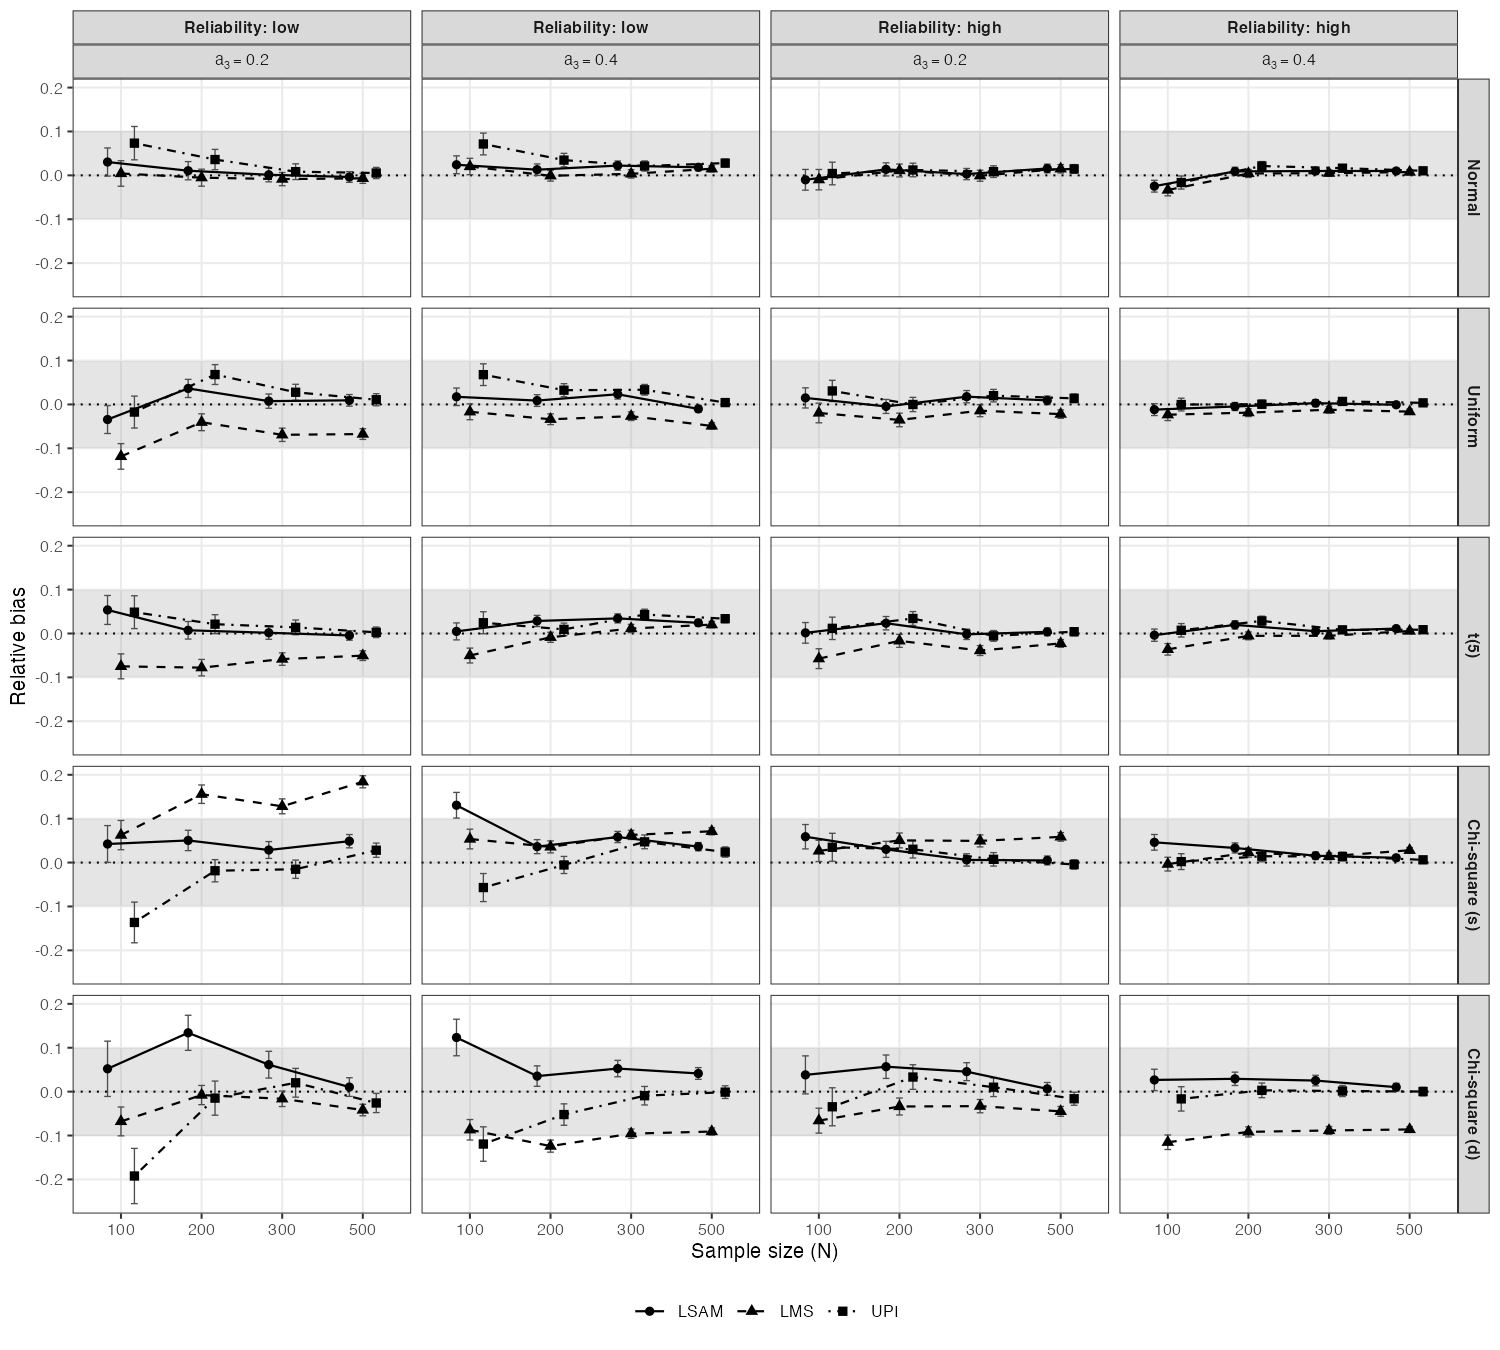
\includegraphics[width=1\linewidth,height=\textheight,keepaspectratio]{../plots/baseline_rel_bias_imm.png}

\vspace{-20pt}
\noindent \emph{Note.} The~gray band marks the acceptable region for the
measure, and the error bars represent the Monte Carlo standard error
(MCSE). imm = index of moderated mediation; LSAM = local
structural-after-measurement; LMS = latent moderated structural
equations; UPI = unconstrained product indicator.

\end{figure}

\begin{figure}[!htbp]

{\caption{{Relative Bias of the Interaction Coefficient (\(a_3\)) Under
the Correctly Specified Condition Across Sample Sizes, Reliability,
Interaction Values, and Distributions}{\label{fig-baseline-bias-a3}}}}

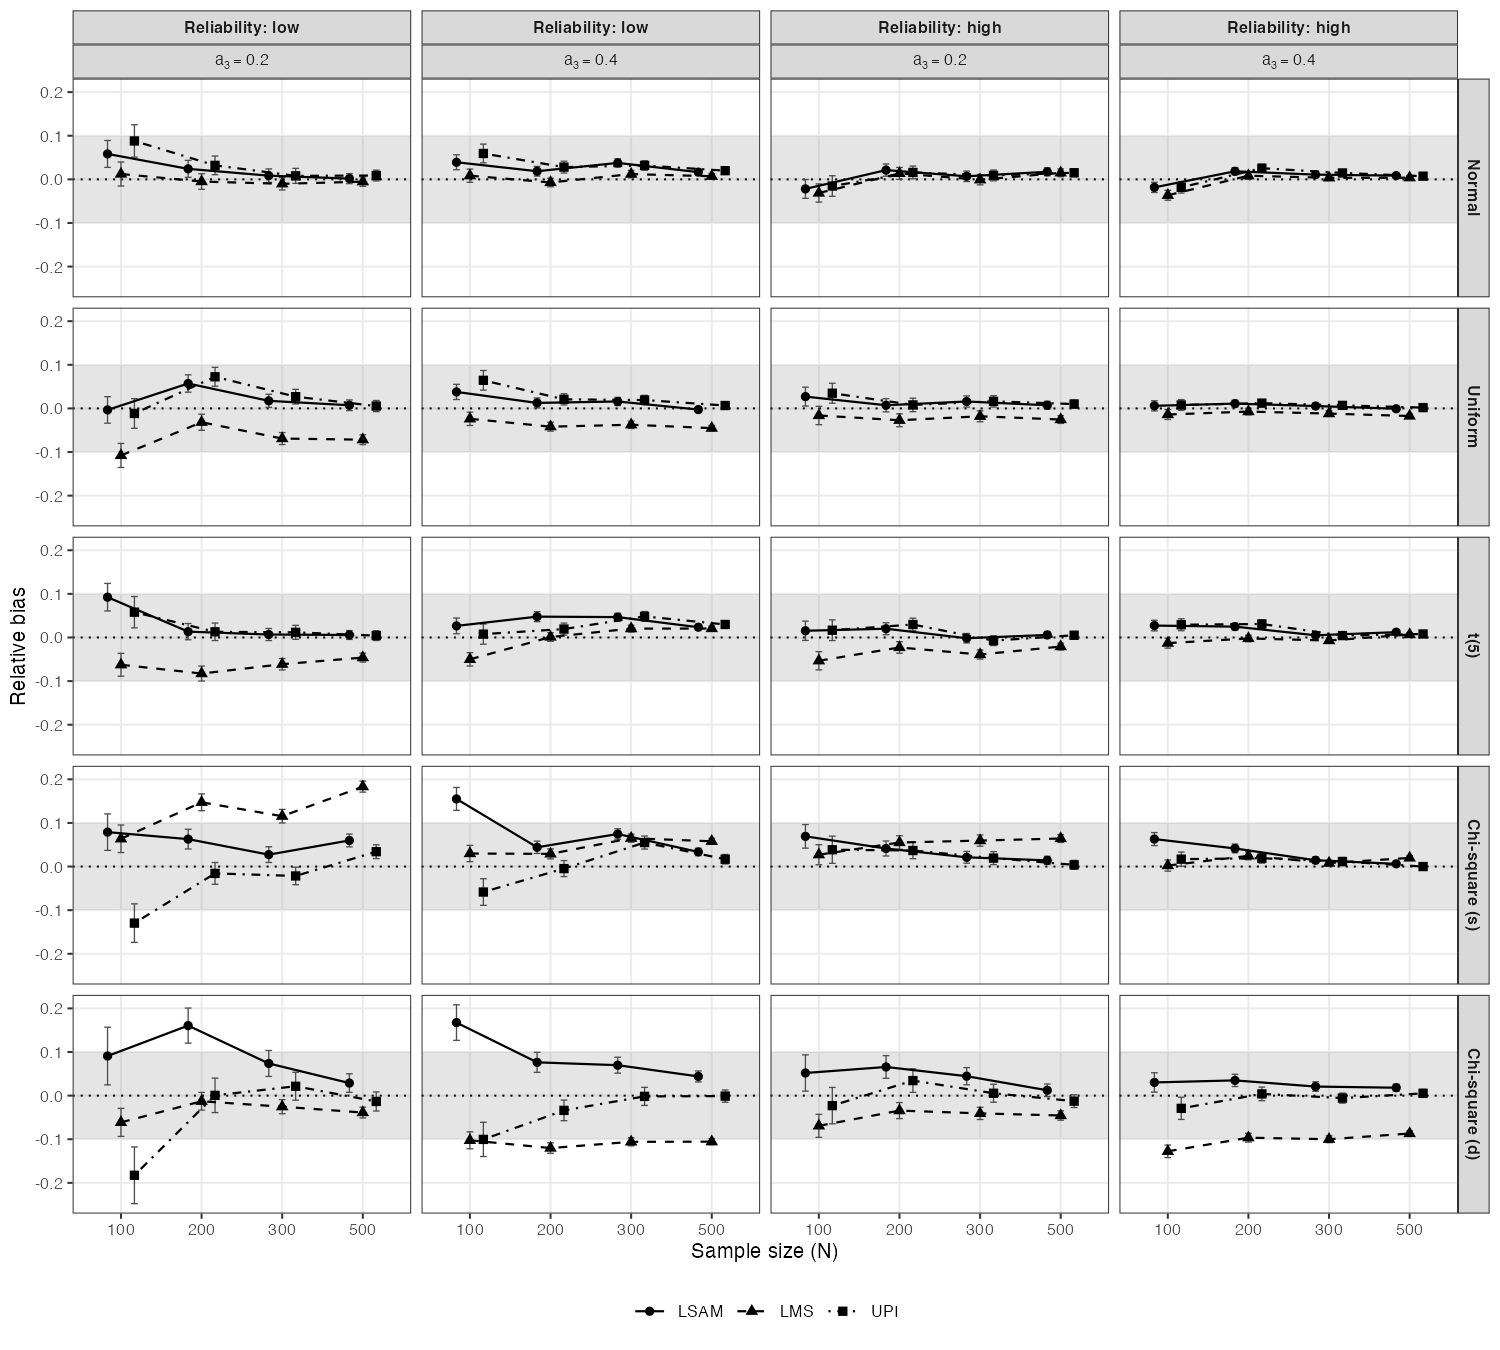
\includegraphics[width=1\linewidth,height=\textheight,keepaspectratio]{../plots/baseline_rel_bias_a3.png}

\vspace{-20pt}
\noindent \emph{Note.} The~gray band marks the acceptable region for the
measure, and the error bars represent the Monte Carlo standard error
(MCSE). LSAM = local structural-after-measurement; LMS = latent
moderated structural equations; UPI = unconstrained product indicator.

\end{figure}

\begin{figure}[!htbp]

{\caption{{Relative Bias of the imm (\(a_3 b\)) and the Interaction
Coefficient (\(a_3\)) Across Distributions, Reliability, and
(Mis)specifications for \(N = 200\) and \(500\) at
\(a_3 = 0.2\)}{\label{fig-bias}}}}

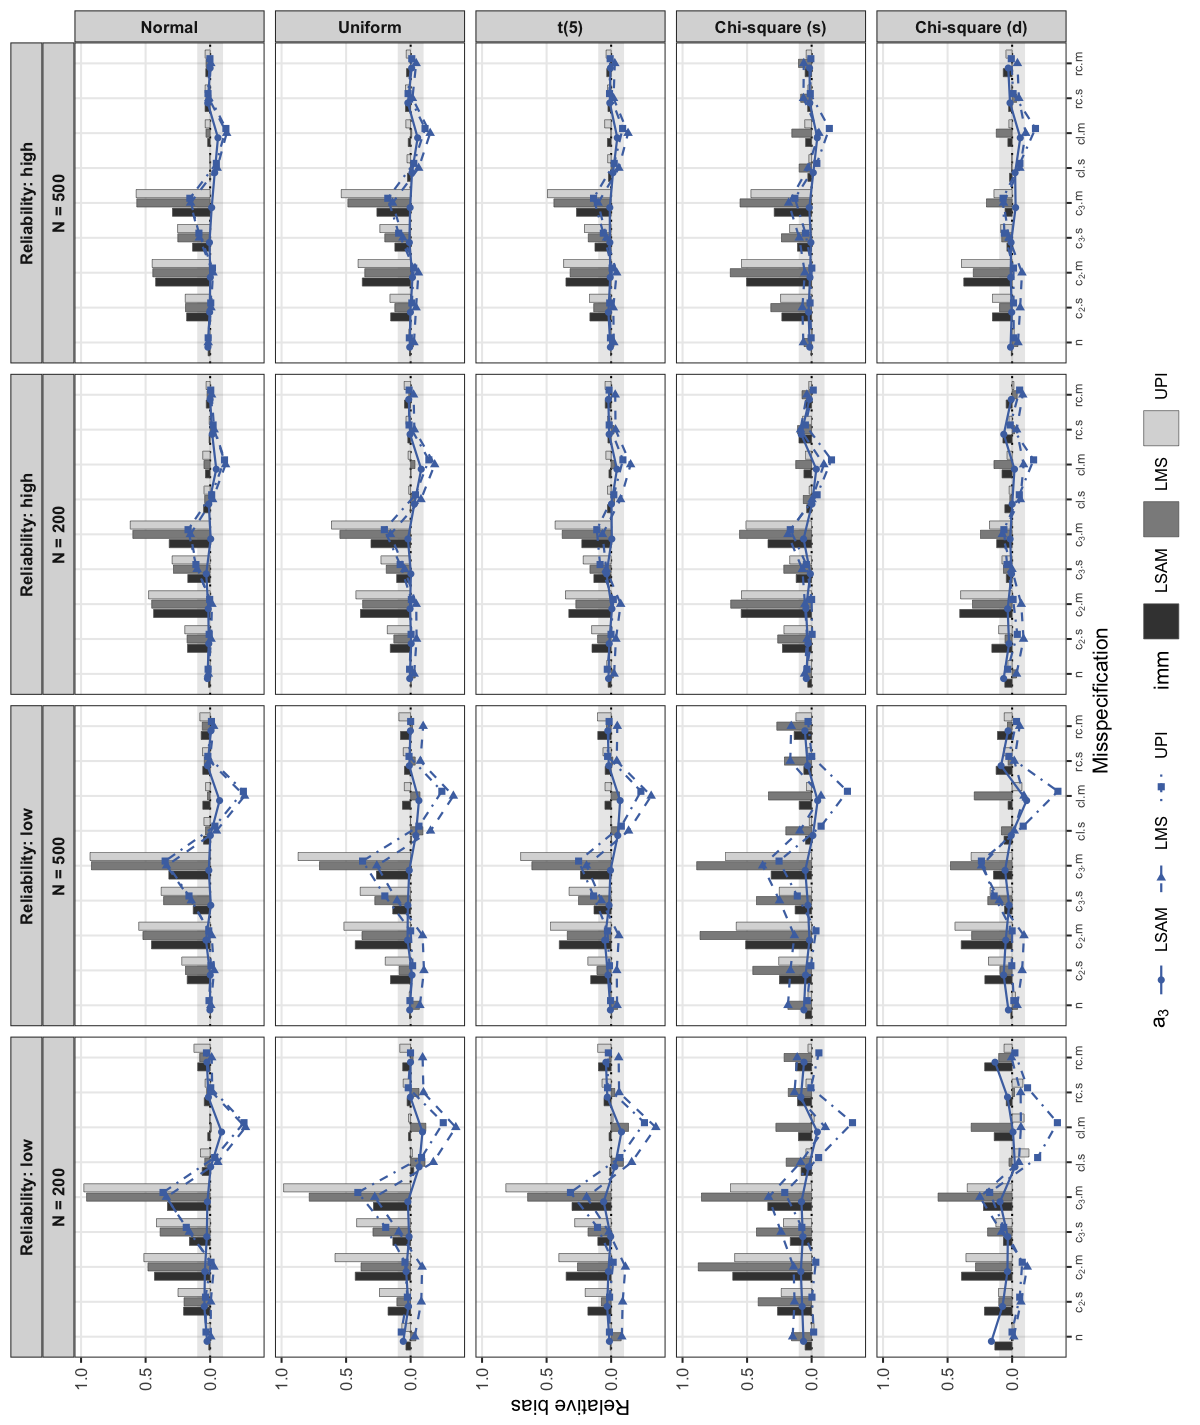
\includegraphics[width=6.3in,height=\textheight,keepaspectratio]{../plots/combo_rel_bias_a3-0.2.png}

\vspace{-20pt}
\noindent \emph{Note.} The~gray band marks the acceptable region for
relative bias. Monte Carlo standard errors (MCSEs) are not shown. imm =
index of moderated mediation; LSAM = local structural-after-measurement;
LMS = latent moderated structural equations; UPI = unconstrained product
indicator; n = no misspecification.

\end{figure}

\begin{figure}[!htbp]

{\caption{{Relative RMSE of the imm (\(a_3 b\)) and the Interaction
Coefficient (\(a_3\)) Across Distributions, Reliability, and
(Mis)specifications for \(N = 200\) and \(500\) at
\(a_3 = 0.2\)}{\label{fig-rmse}}}}

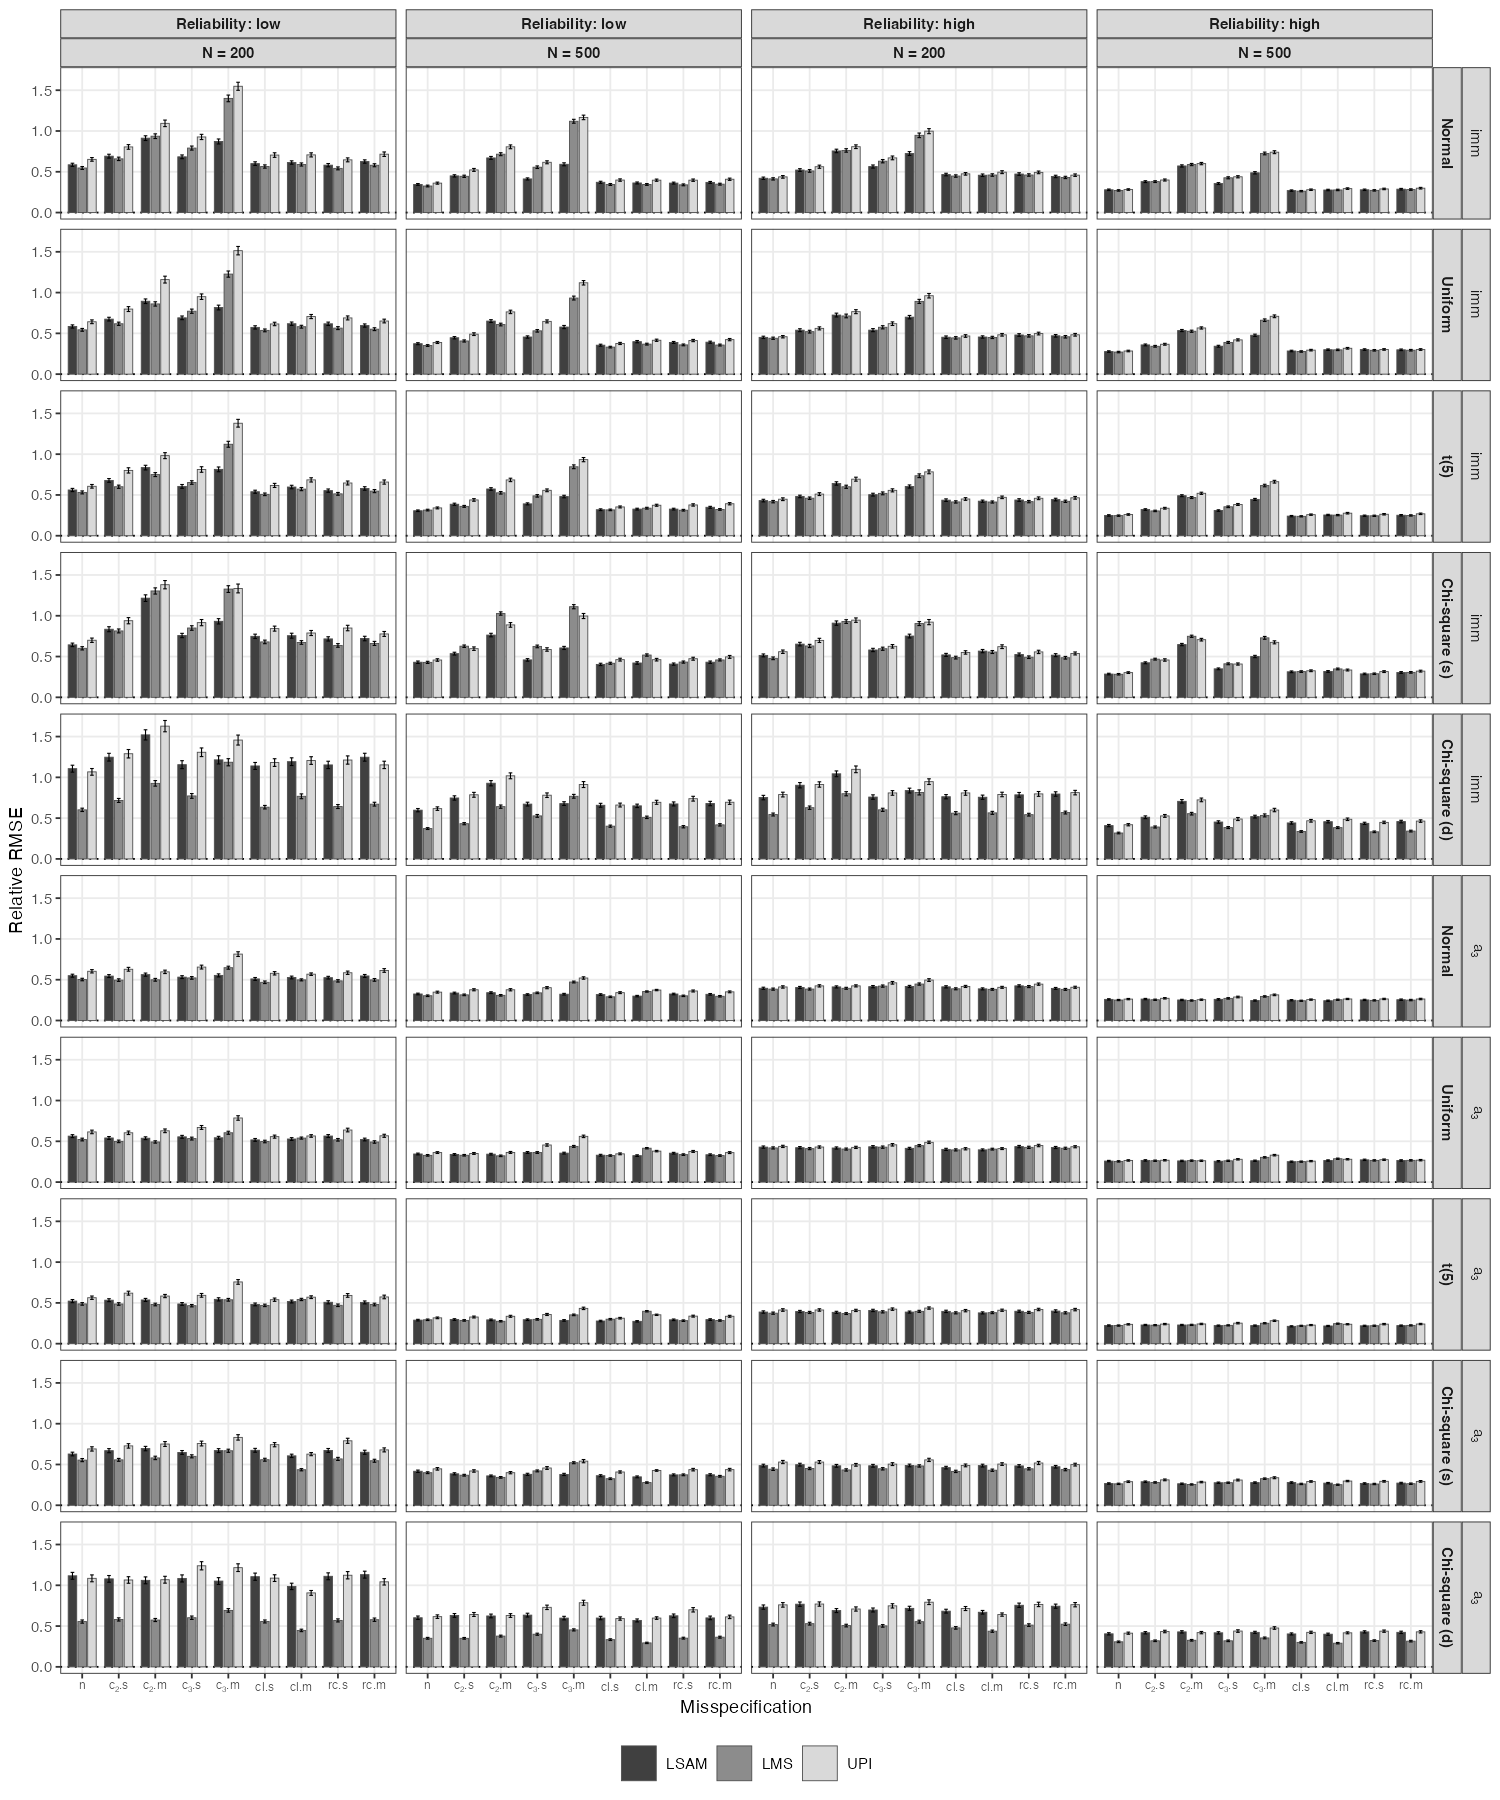
\includegraphics[width=1\linewidth,height=\textheight,keepaspectratio]{../plots/both_rel_rmse_a3-0.2.png}

\vspace{-20pt}
\noindent \emph{Note.} The~error bars represent the Monte Carlo standard
error (MCSE). No acceptable region is defined for this measure. imm =
index of moderated mediation; LSAM = local structural-after-measurement;
LMS = latent moderated structural equations; UPI = unconstrained product
indicator; n = no misspecification.

\end{figure}

\begin{figure}[!htbp]

{\caption{{SE/SD of the imm (\(a_3 b\)) Across Distributions,
Reliability, and (Mis)specifications for \(N = 200\) and \(500\) at
\(a_3 = 0.2\)}{\label{fig-sesd-imm}}}}

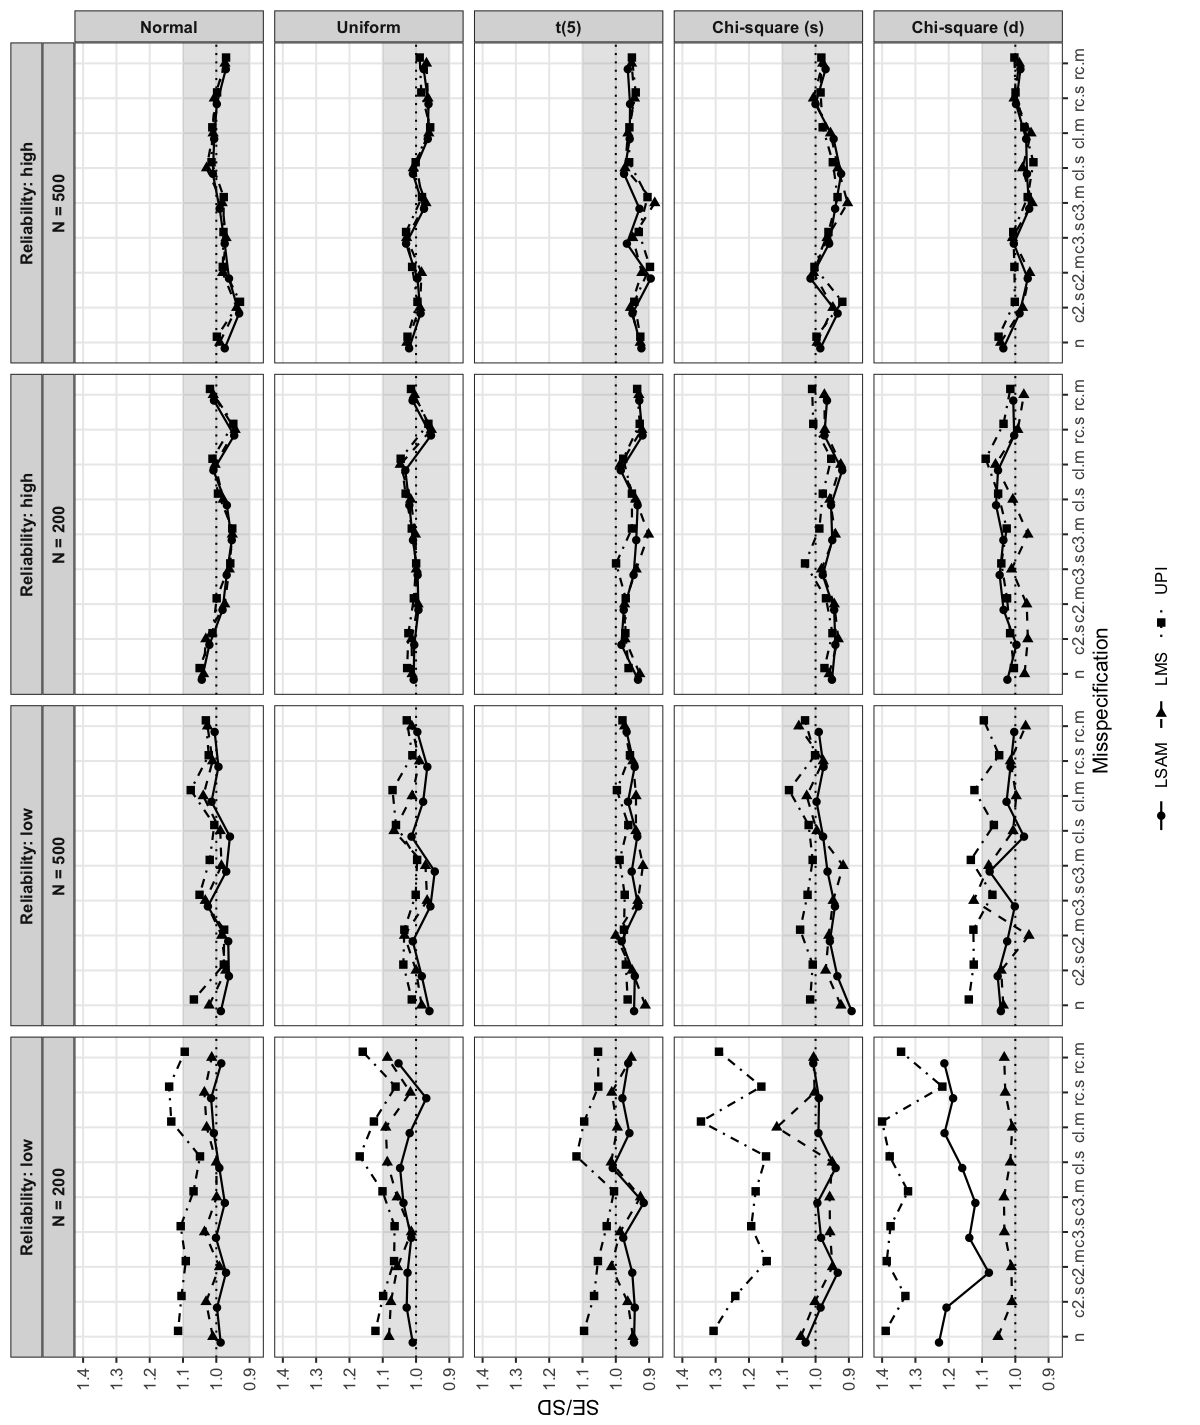
\includegraphics[width=6.3in,height=\textheight,keepaspectratio]{../plots/imm_se_sd_a3-0.2_byrel.png}

\vspace{-20pt}
\noindent \emph{Note.} The~gray band marks the acceptable region for the
measure. The Monte Carlo standard error (MCSE) is not computed for the
SE/SD ratio. imm = index of moderated mediation; LSAM = local
structural-after-measurement; LMS = latent moderated structural
equations; UPI = unconstrained product indicator; n = no
misspecification.

\end{figure}

\begin{figure}[!htbp]

{\caption{{SE/SD of the Interaction Coefficient (\(a_3\)) Across
Distributions, Reliability, and (Mis)specifications for \(N = 200\) and
\(500\) at \(a_3 = 0.2\)}{\label{fig-sesd-a3}}}}

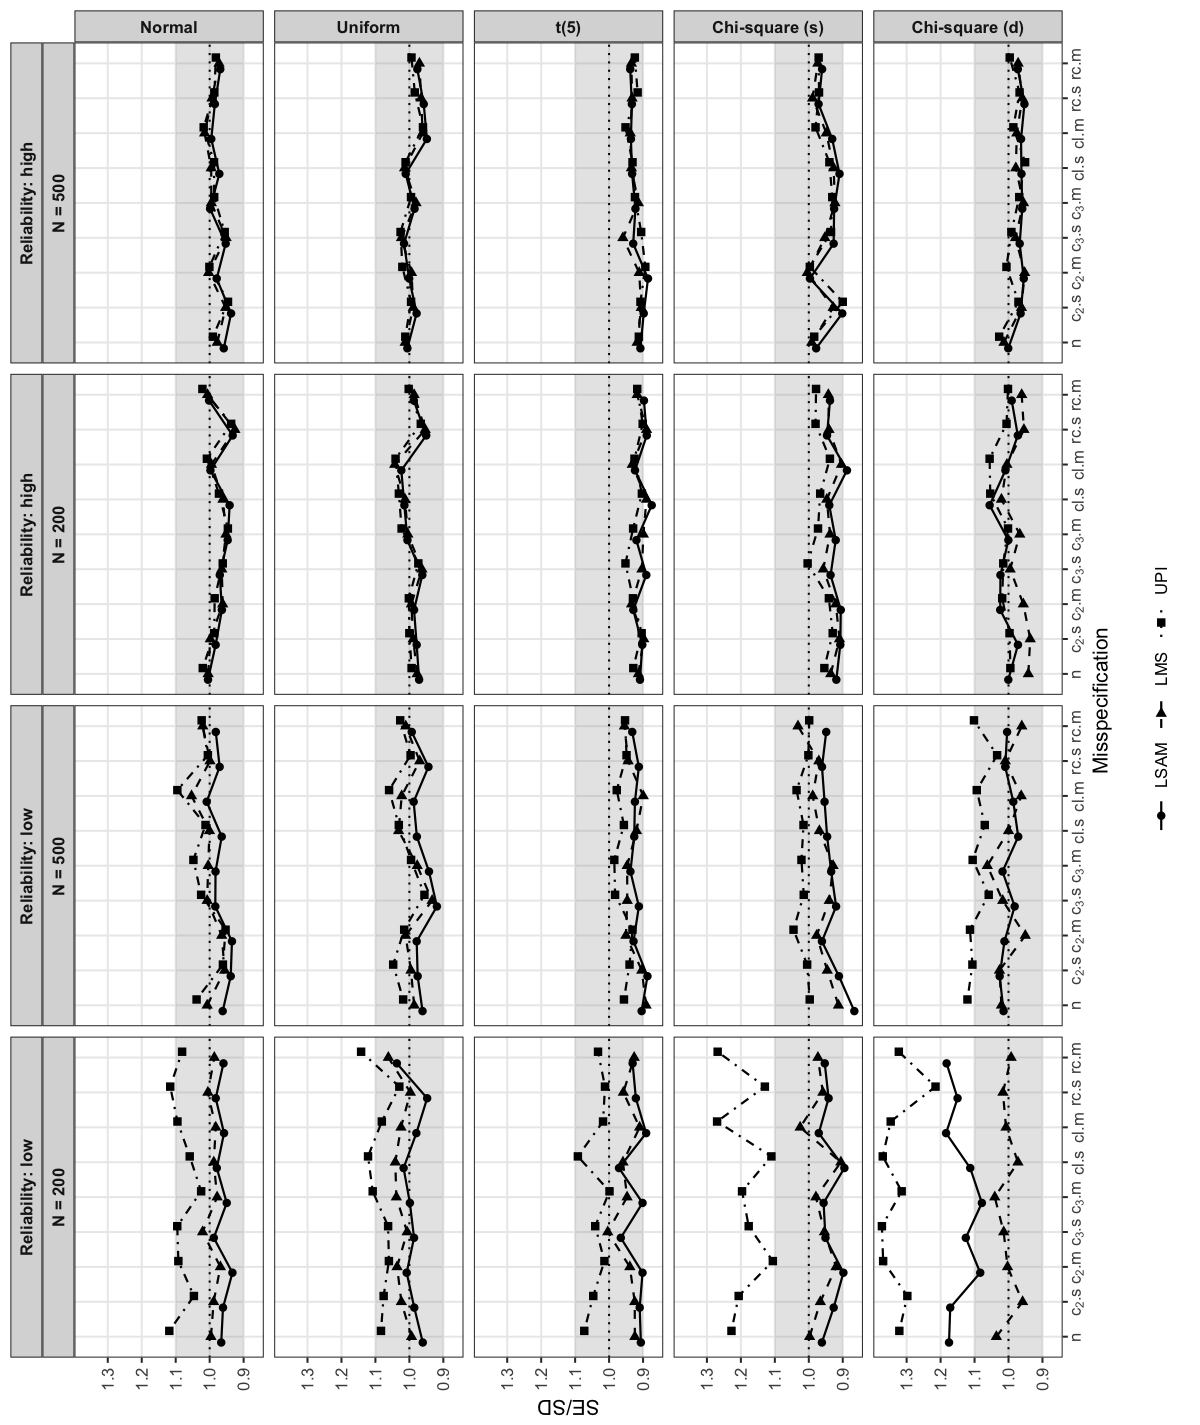
\includegraphics[width=6.3in,height=\textheight,keepaspectratio]{../plots/a3_se_sd_a3-0.2_byrel.png}

\vspace{-20pt}
\noindent \emph{Note.} The~gray band marks the acceptable region for the
measure. The Monte Carlo standard error (MCSE) is not computed for the
SE/SD ratio. LSAM = local structural-after-measurement; LMS = latent
moderated structural equations; UPI = unconstrained product indicator; n
= no misspecification.

\end{figure}

\begin{figure}[!htbp]

{\caption{{Coverage of the imm (\(a_3 b\)) Across Distributions,
Reliability, and (Mis)specifications for \(N = 200\) and \(500\) at
\(a_3 = 0.2\)}{\label{fig-coverage-imm}}}}

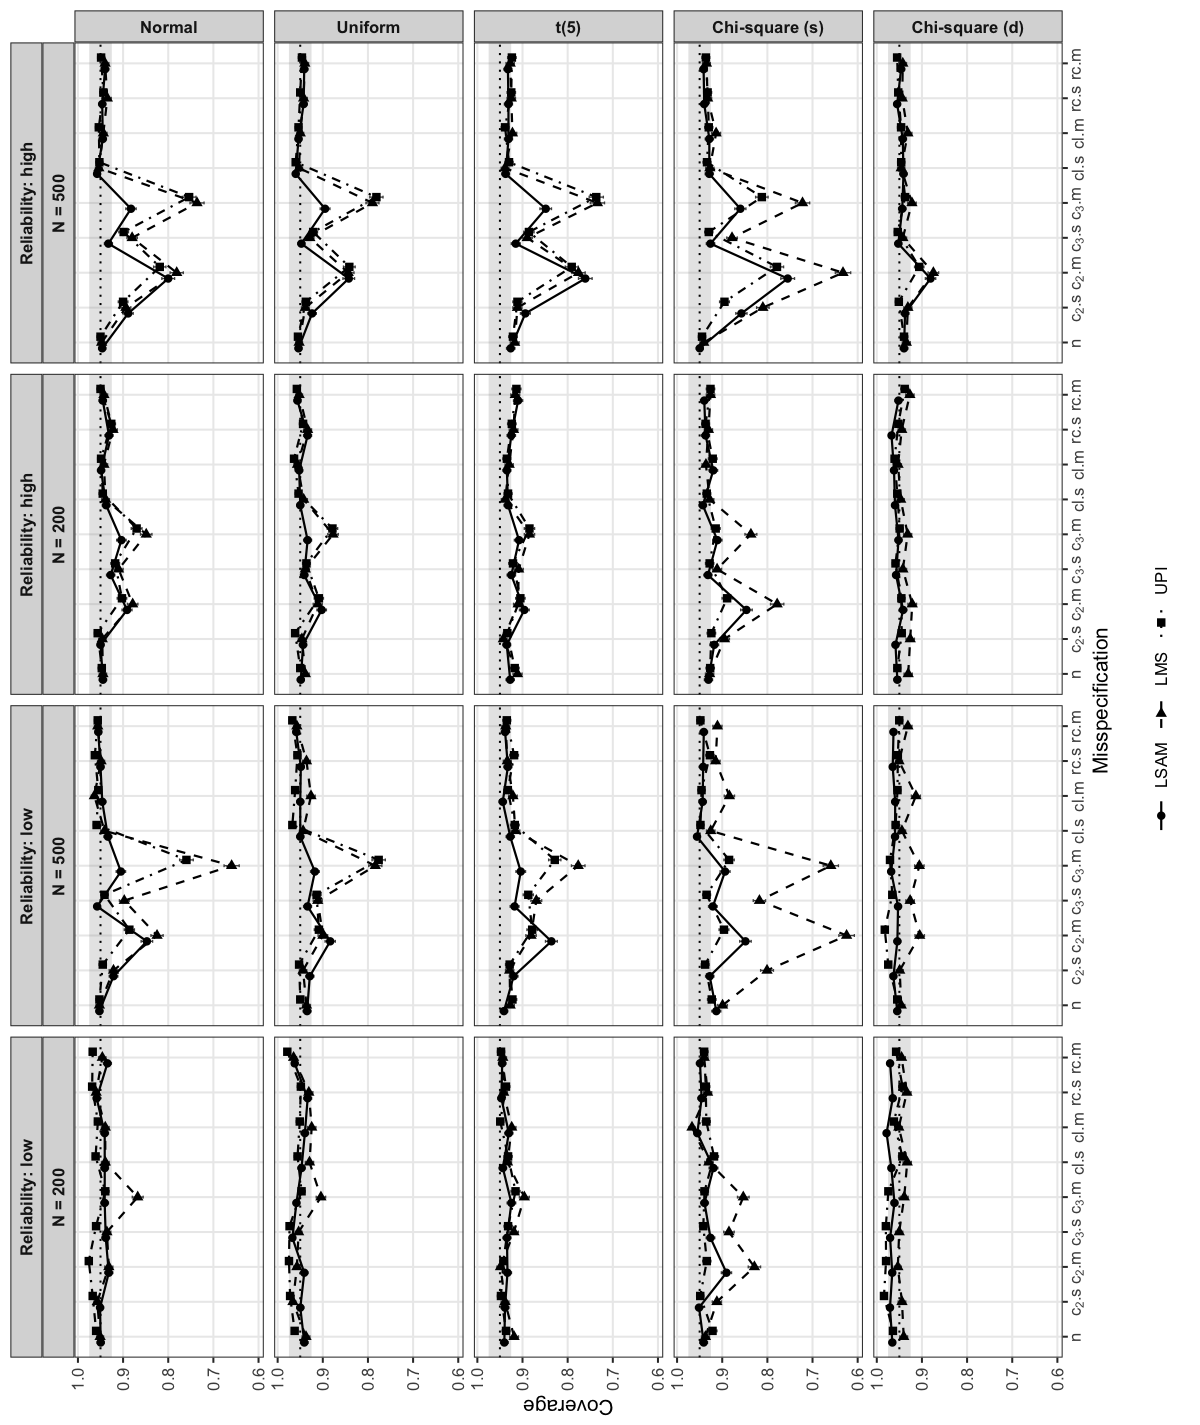
\includegraphics[width=6.3in,height=\textheight,keepaspectratio]{../plots/imm_coverage_a3-0.2_byrel.png}

\vspace{-20pt}
\noindent \emph{Note.} The~gray band marks the acceptable region for the
measure, and the error bars represent the Monte Carlo standard error
(MCSE). imm = index of moderated mediation; LSAM = local
structural-after-measurement; LMS = latent moderated structural
equations; UPI = unconstrained product indicator; n = no
misspecification.

\end{figure}

\begin{figure}[!htbp]

{\caption{{Coverage of the Interaction Coefficient (\(a_3\)) Across
Distributions, Reliability, and (Mis)specifications for \(N = 200\) and
\(500\) at \(a_3 = 0.2\)}{\label{fig-coverage-a3}}}}

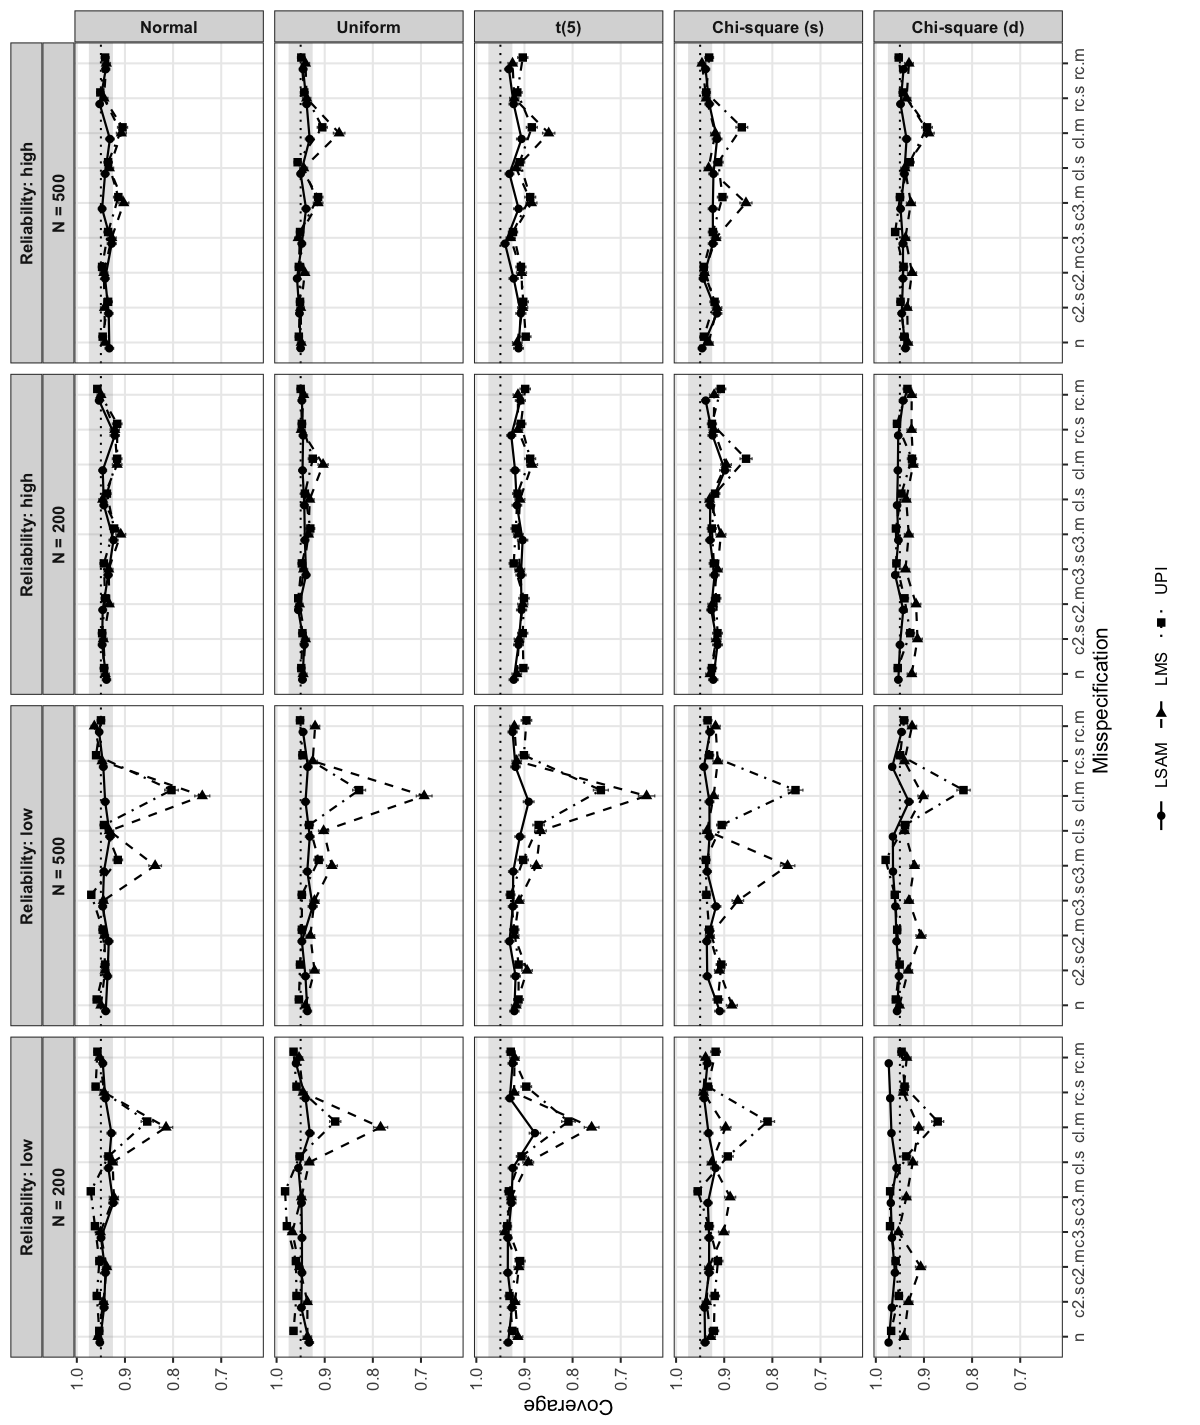
\includegraphics[width=6.3in,height=\textheight,keepaspectratio]{../plots/a3_coverage_a3-0.2_byrel.png}

\vspace{-20pt}
\noindent \emph{Note.} The~gray band marks the acceptable region for the
measure, and the error bars represent the Monte Carlo standard error
(MCSE). LSAM = local structural-after-measurement; LMS = latent
moderated structural equations; UPI = unconstrained product indicator; n
= no misspecification.

\end{figure}

\begin{figure}[!htbp]

{\caption{{Type I Error of the imm (\(a_3 b\)) and the Interaction
Coefficient (\(a_3\)) Across Distributions, Reliability, and
(Mis)specifications for \(N = 200\) and \(500\) at
\(a_3 = 0\)}{\label{fig-typei}}}}

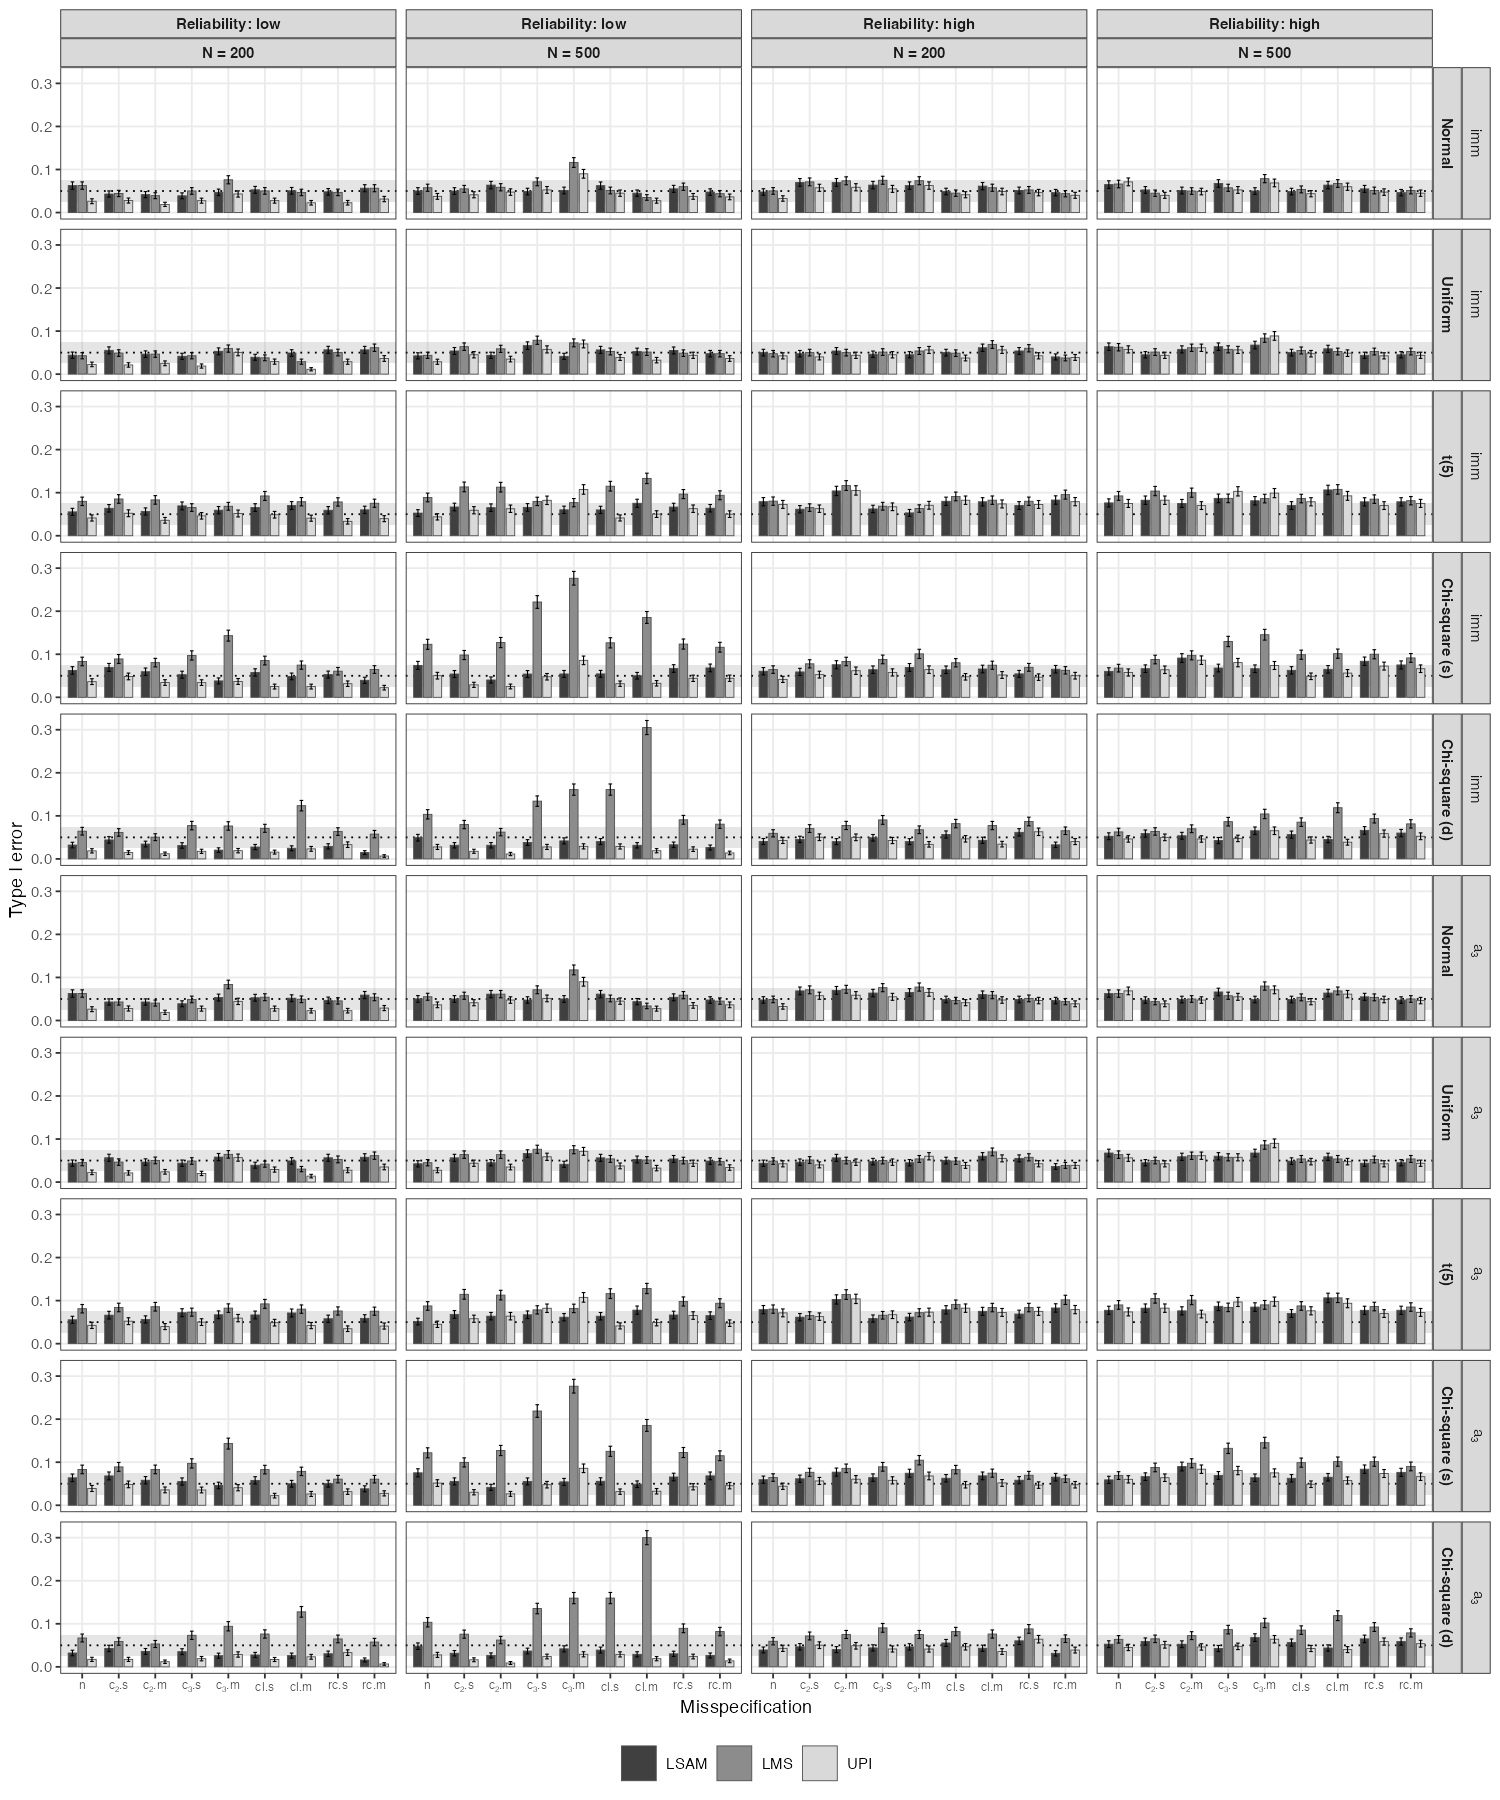
\includegraphics[width=1\linewidth,height=\textheight,keepaspectratio]{../plots/both_typeI_a3-0.png}

\vspace{-20pt}
\noindent \emph{Note.} The~gray band marks the acceptable region for the
measure, and the error bars represent the Monte Carlo standard error
(MCSE). imm = index of moderated mediation; LSAM = local
structural-after-measurement; LMS = latent moderated structural
equations; UPI = unconstrained product indicator; n = no
misspecification.

\end{figure}

\begin{figure}[!htbp]

{\caption{{Power for the imm (\(a_3 b\)) and the Interaction Coefficient
(\(a_3\)) Across Distributions, Reliability, and (Mis)specifications for
\(N = 200\) and \(500\) at \(a_3 = 0.2\)}{\label{fig-power}}}}

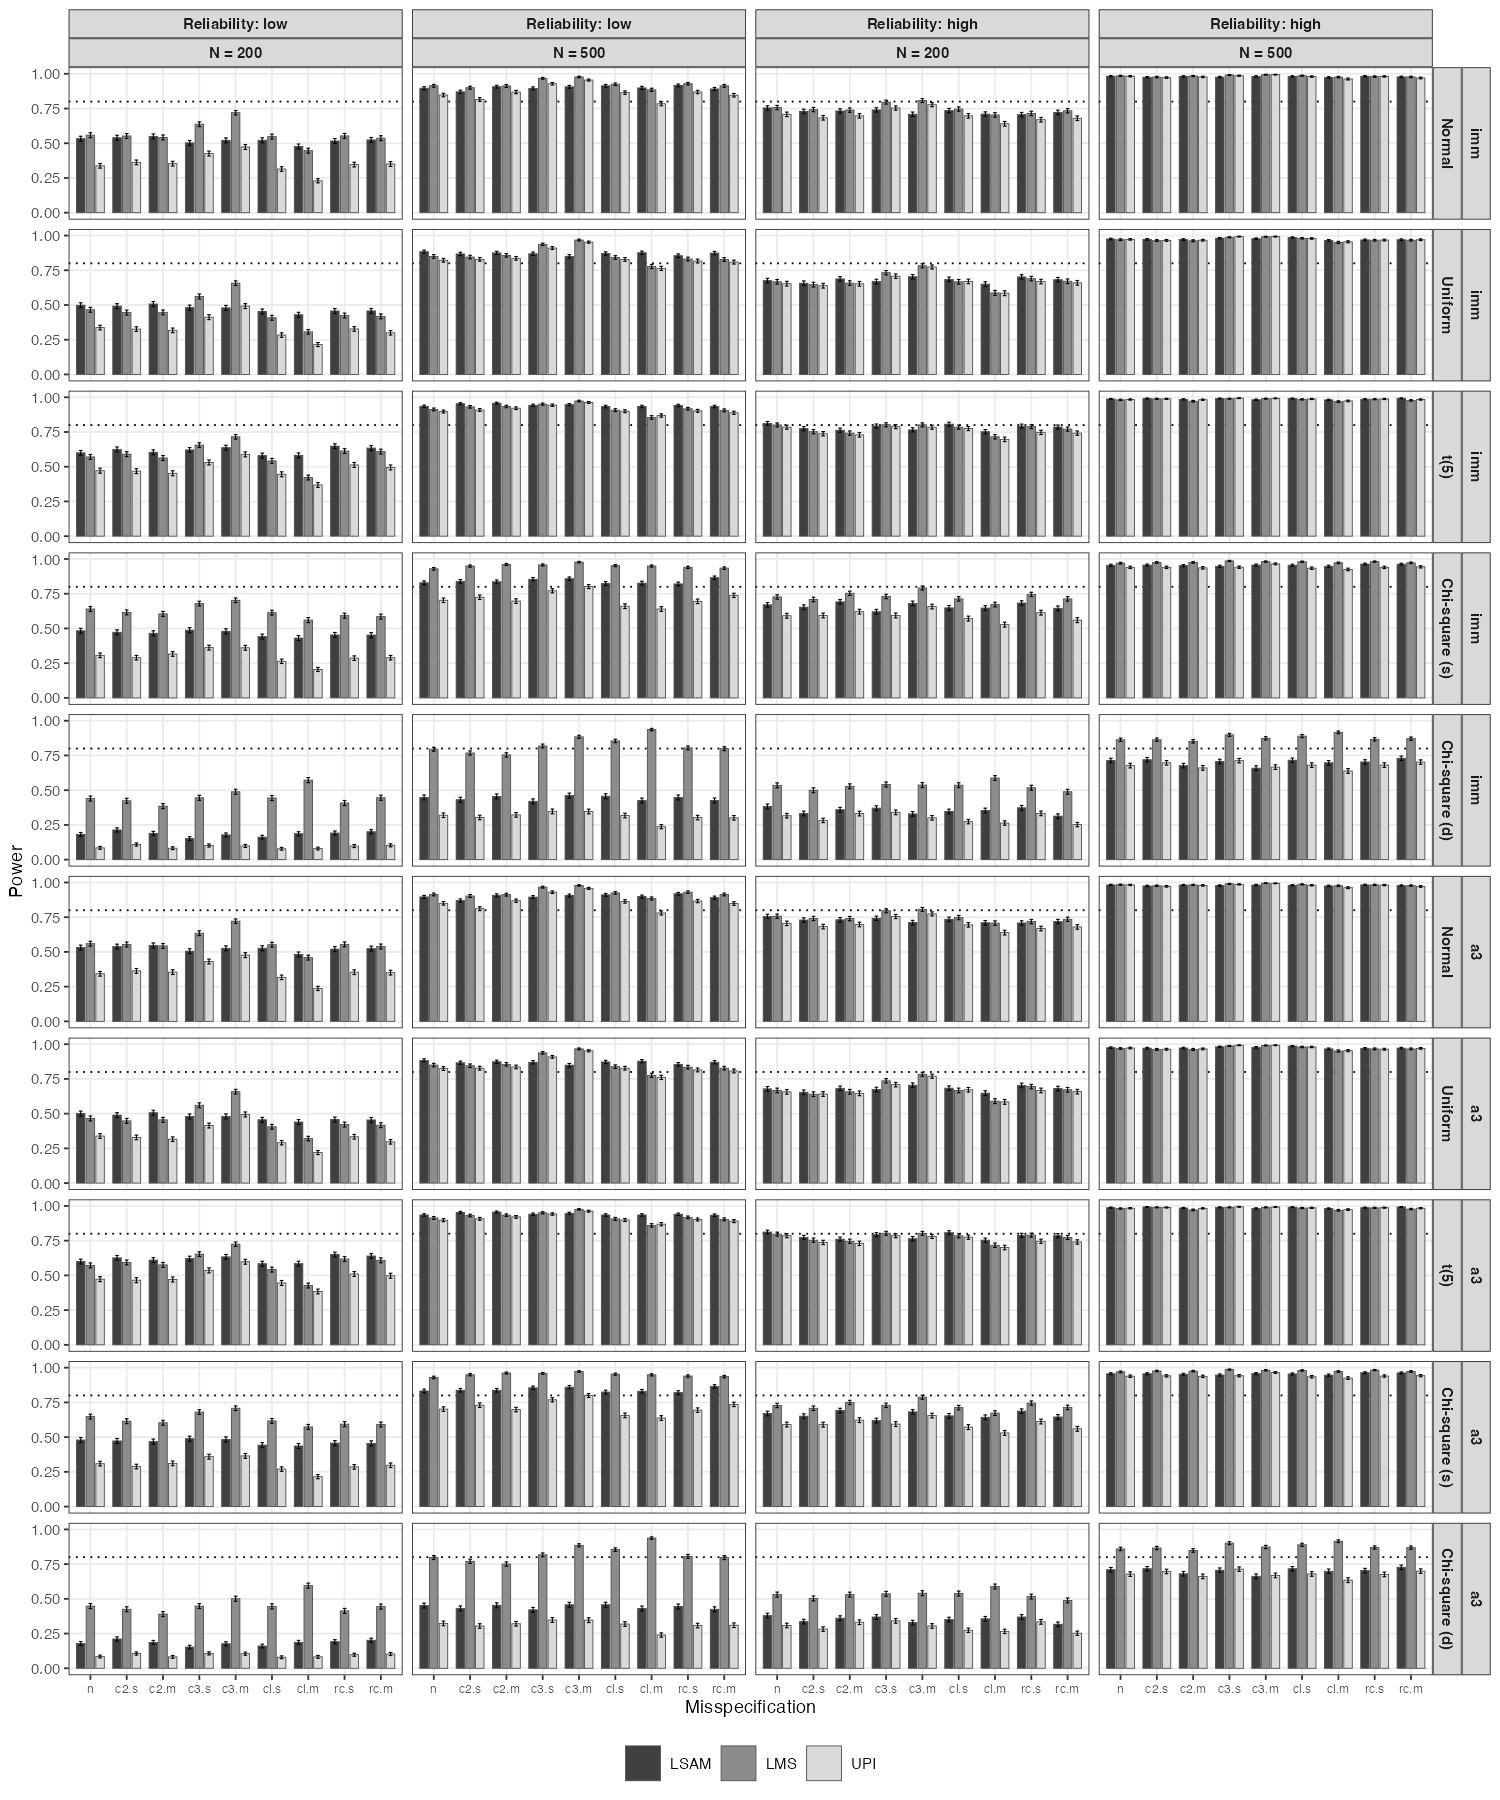
\includegraphics[width=1\linewidth,height=\textheight,keepaspectratio]{../plots/both_power_a3-0.2.png}

\vspace{-20pt}
\noindent \emph{Note.} The~error bars represent the Monte Carlo standard
error (MCSE). No acceptable region is defined for this measure. imm =
index of moderated mediation; LSAM = local structural-after-measurement;
LMS = latent moderated structural equations; UPI = unconstrained product
indicator; n = no misspecification.

\end{figure}

\begin{figure}[!htbp]

{\caption{{Relative Bias of the Structural Coefficients (\(a_1\),
\(a_2\), \(b\), \(c'\)) Across Distributions and (Mis)specifications at
High Reliability, \(N = 500\), and
\(a_3 = 0.2\)}{\label{fig-param-bias}}}}

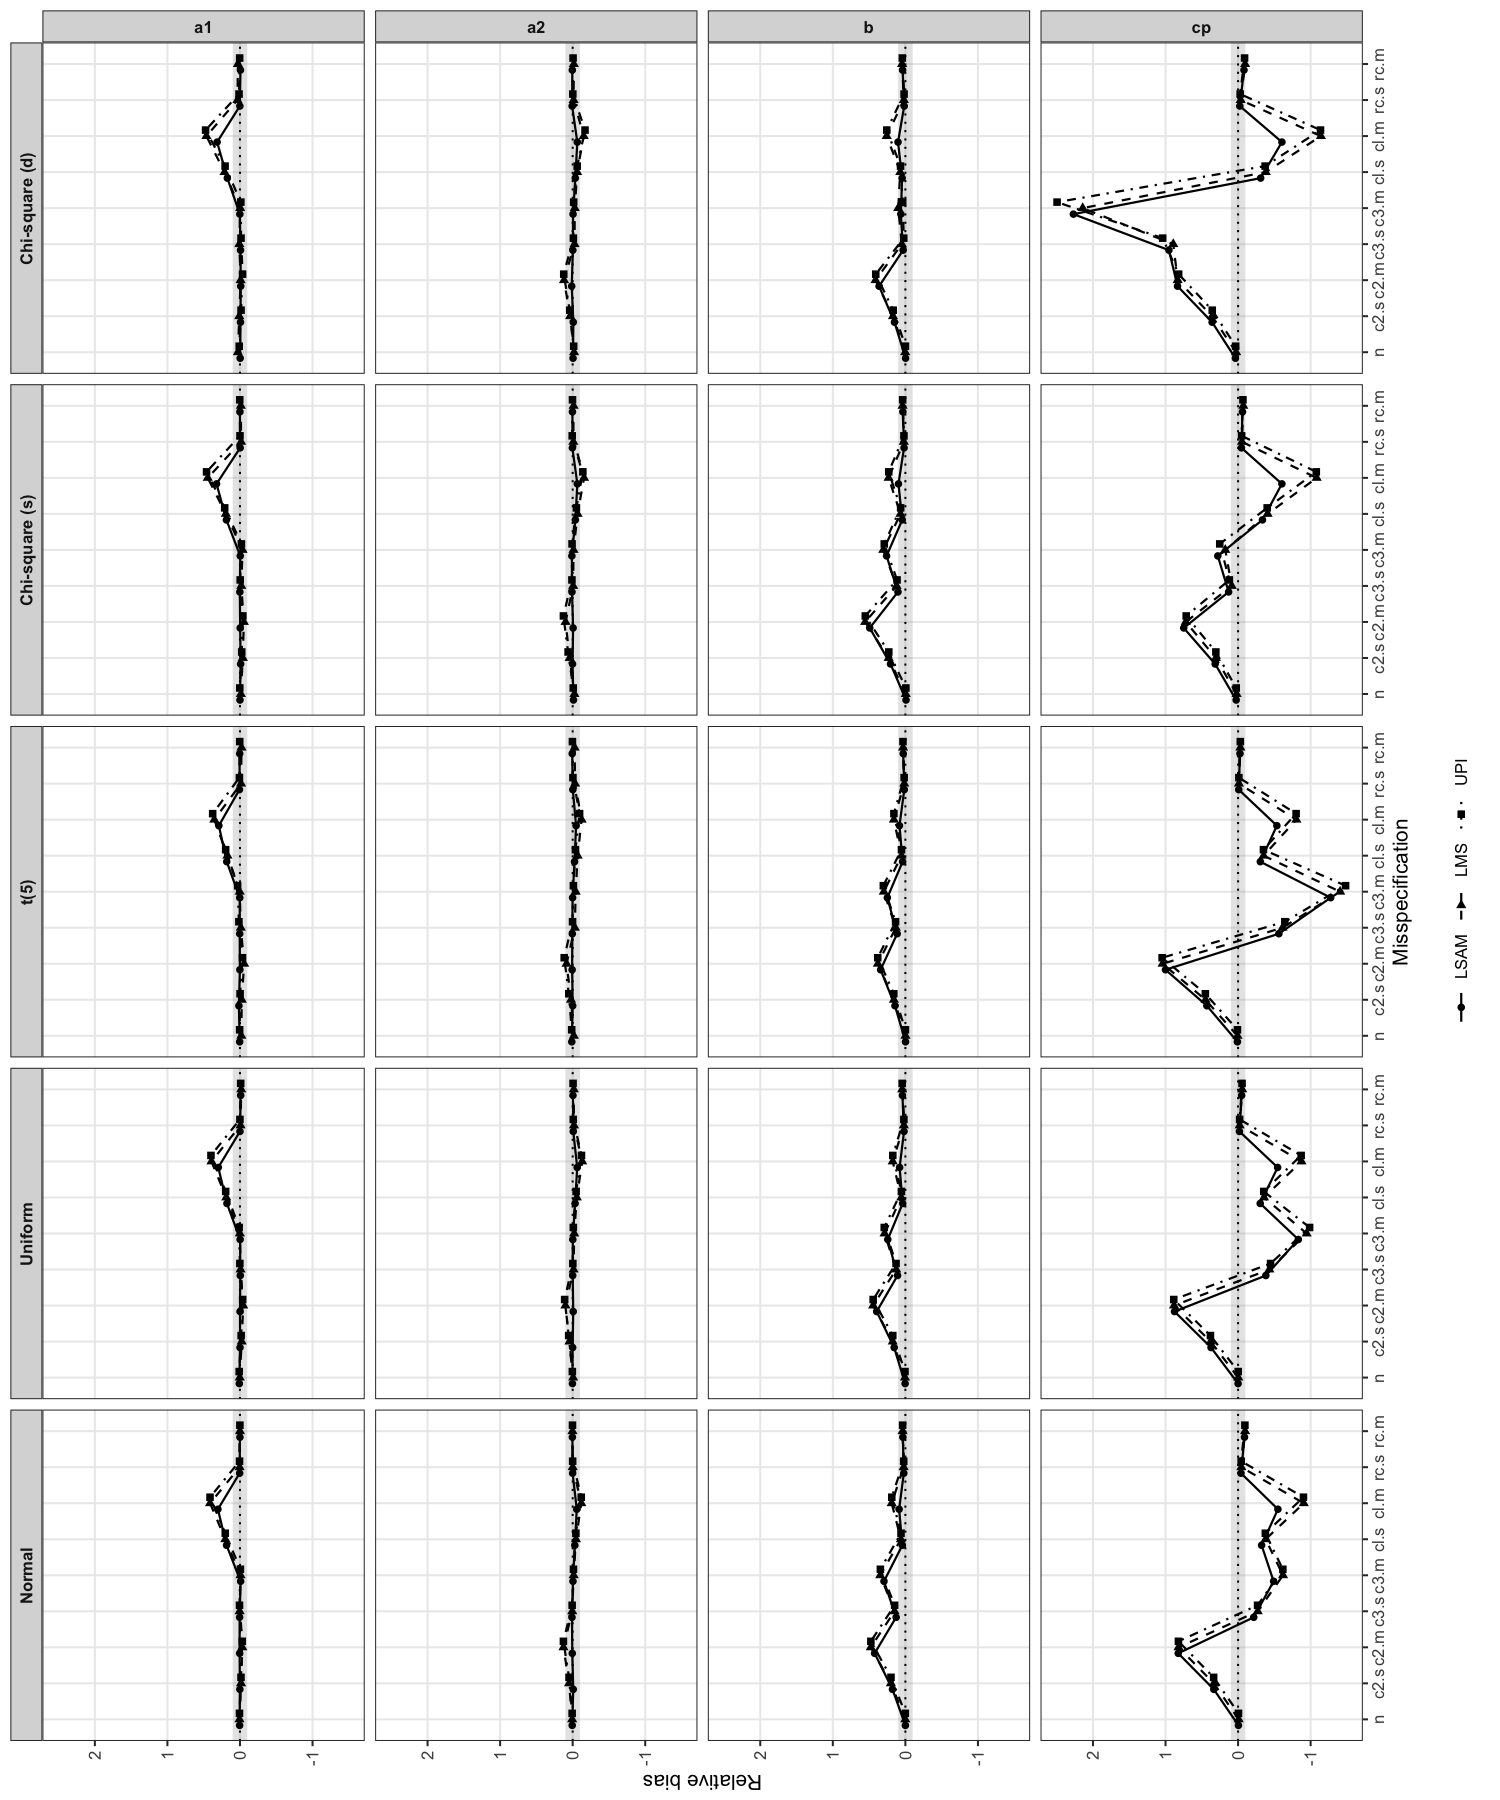
\includegraphics[width=6.3in,height=\textheight,keepaspectratio]{../plots/param_rel_bias_a3-0.2_n500_high.png}

\vspace{-20pt}
\noindent \emph{Note.} The~gray band marks the acceptable region for the
measure, and the error bars represent the Monte Carlo standard error
(MCSE). LSAM = local structural-after-measurement; LMS = latent
moderated structural equations; UPI = unconstrained product indicator; n
= no misspecification.

\end{figure}

\begin{figure}[!htbp]

{\caption{{Coverage of the Structural Coefficients (\(a_1\), \(a_2\),
\(b\), \(c'\)) Across Distributions and (Mis)specifications at High
Reliability, \(N = 500\), and
\(a_3 = 0.2\)}{\label{fig-param-coverage}}}}

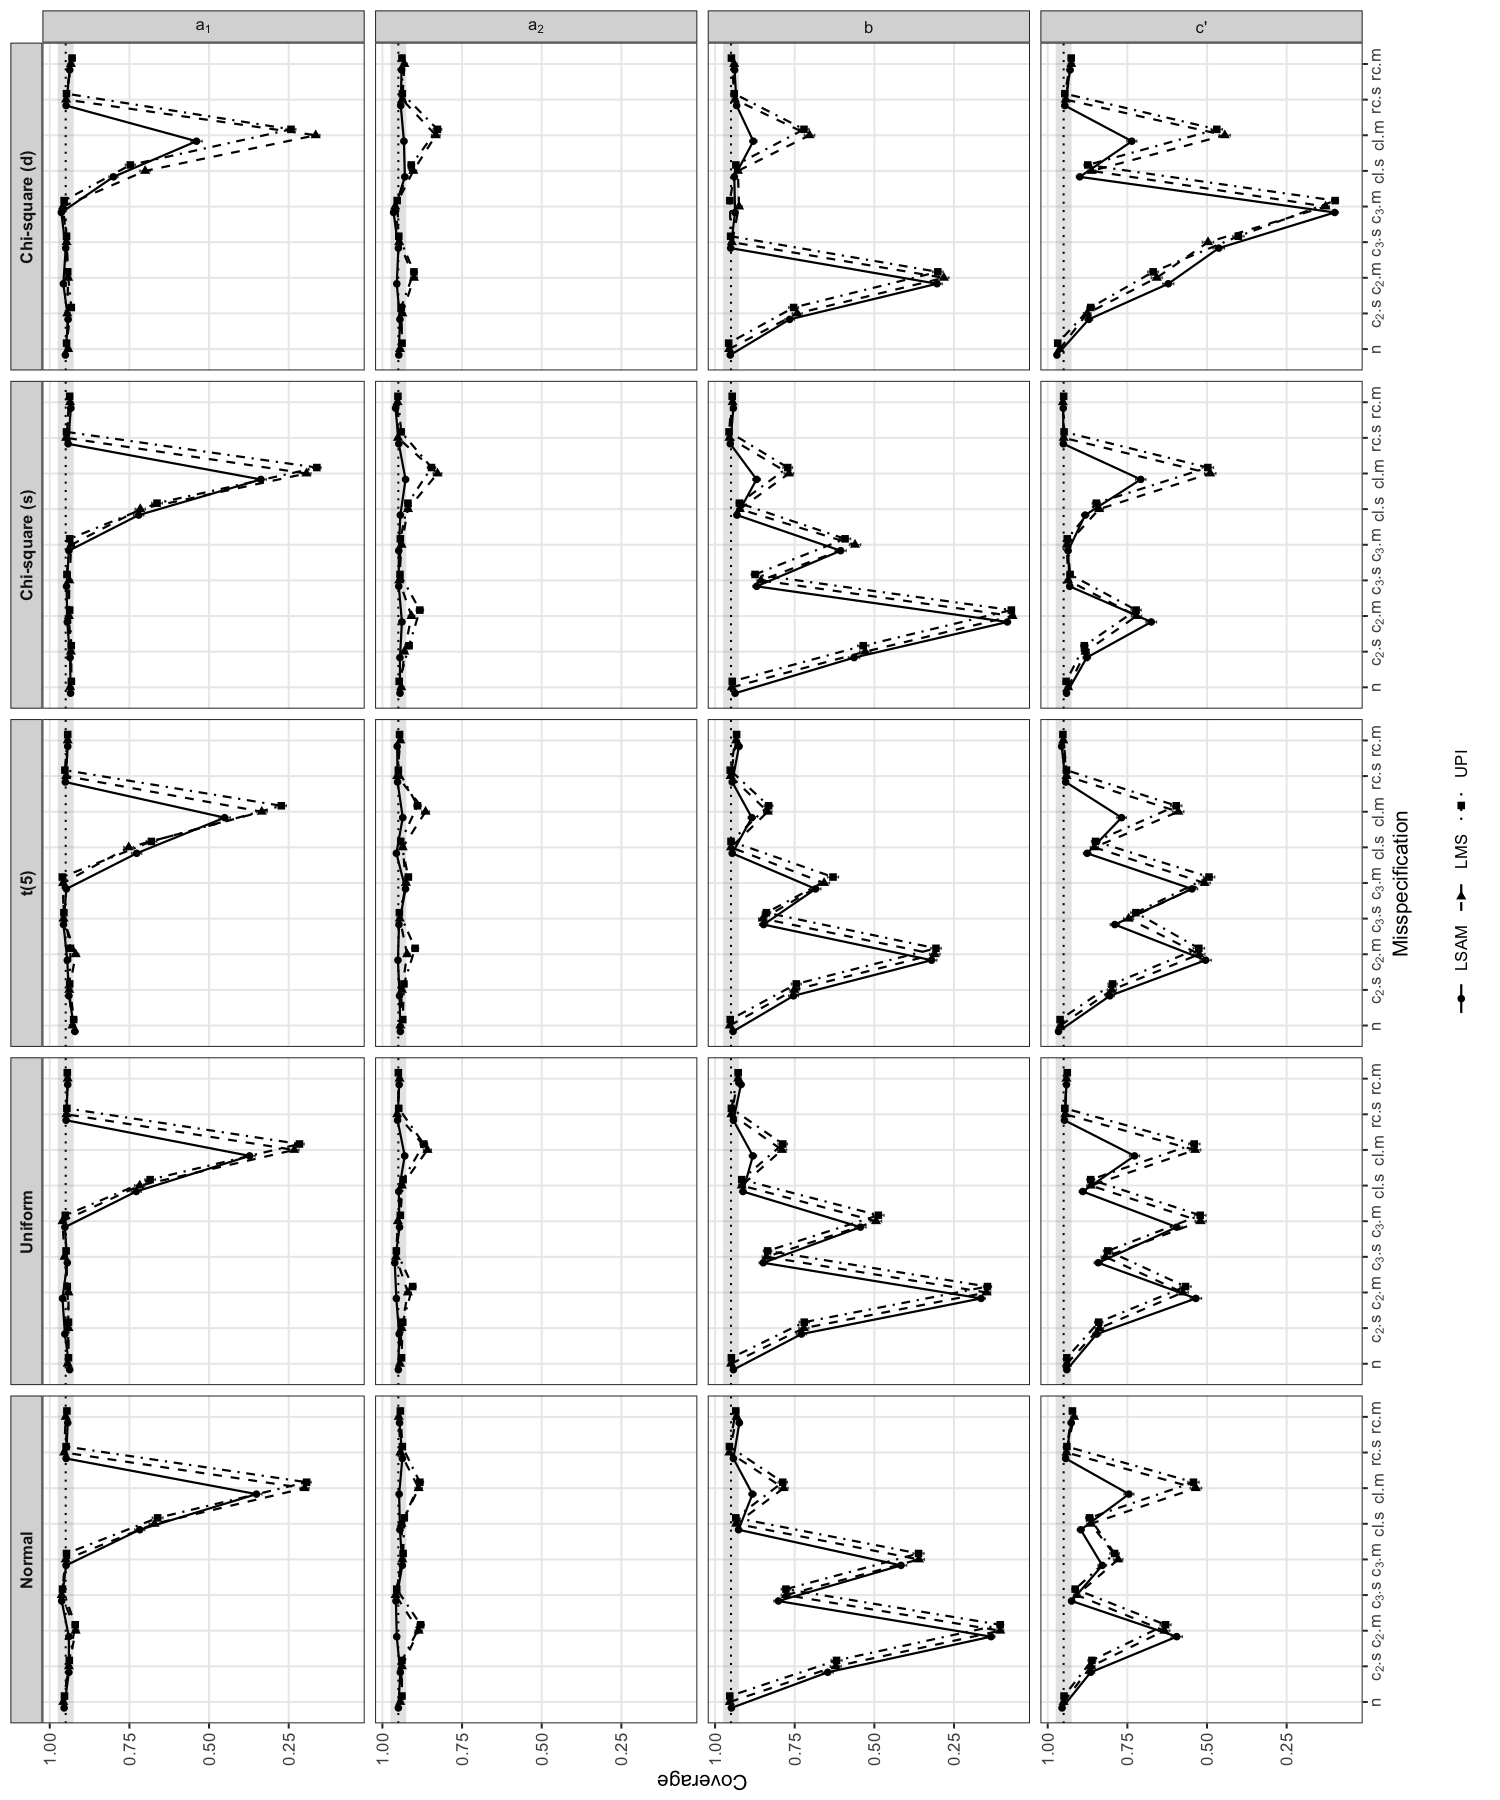
\includegraphics[width=6.3in,height=\textheight,keepaspectratio]{../plots/param_coverage_a3-0.2_n500_high.png}

\vspace{-20pt}
\noindent \emph{Note.} The~gray band marks the acceptable region for the
measure, and the error bars represent the Monte Carlo standard error
(MCSE). LSAM = local structural-after-measurement; LMS = latent
moderated structural equations; UPI = unconstrained product indicator; n
= no misspecification.

\end{figure}

\begin{figure}[!htbp]

{\caption{{SE/SD of the Structural Coefficients (\(a_1\), \(a_2\),
\(b\), \(c'\)) Across Distributions and (Mis)specifications at High
Reliability, \(N = 500\), and \(a_3 = 0.2\)}{\label{fig-param-sesd}}}}

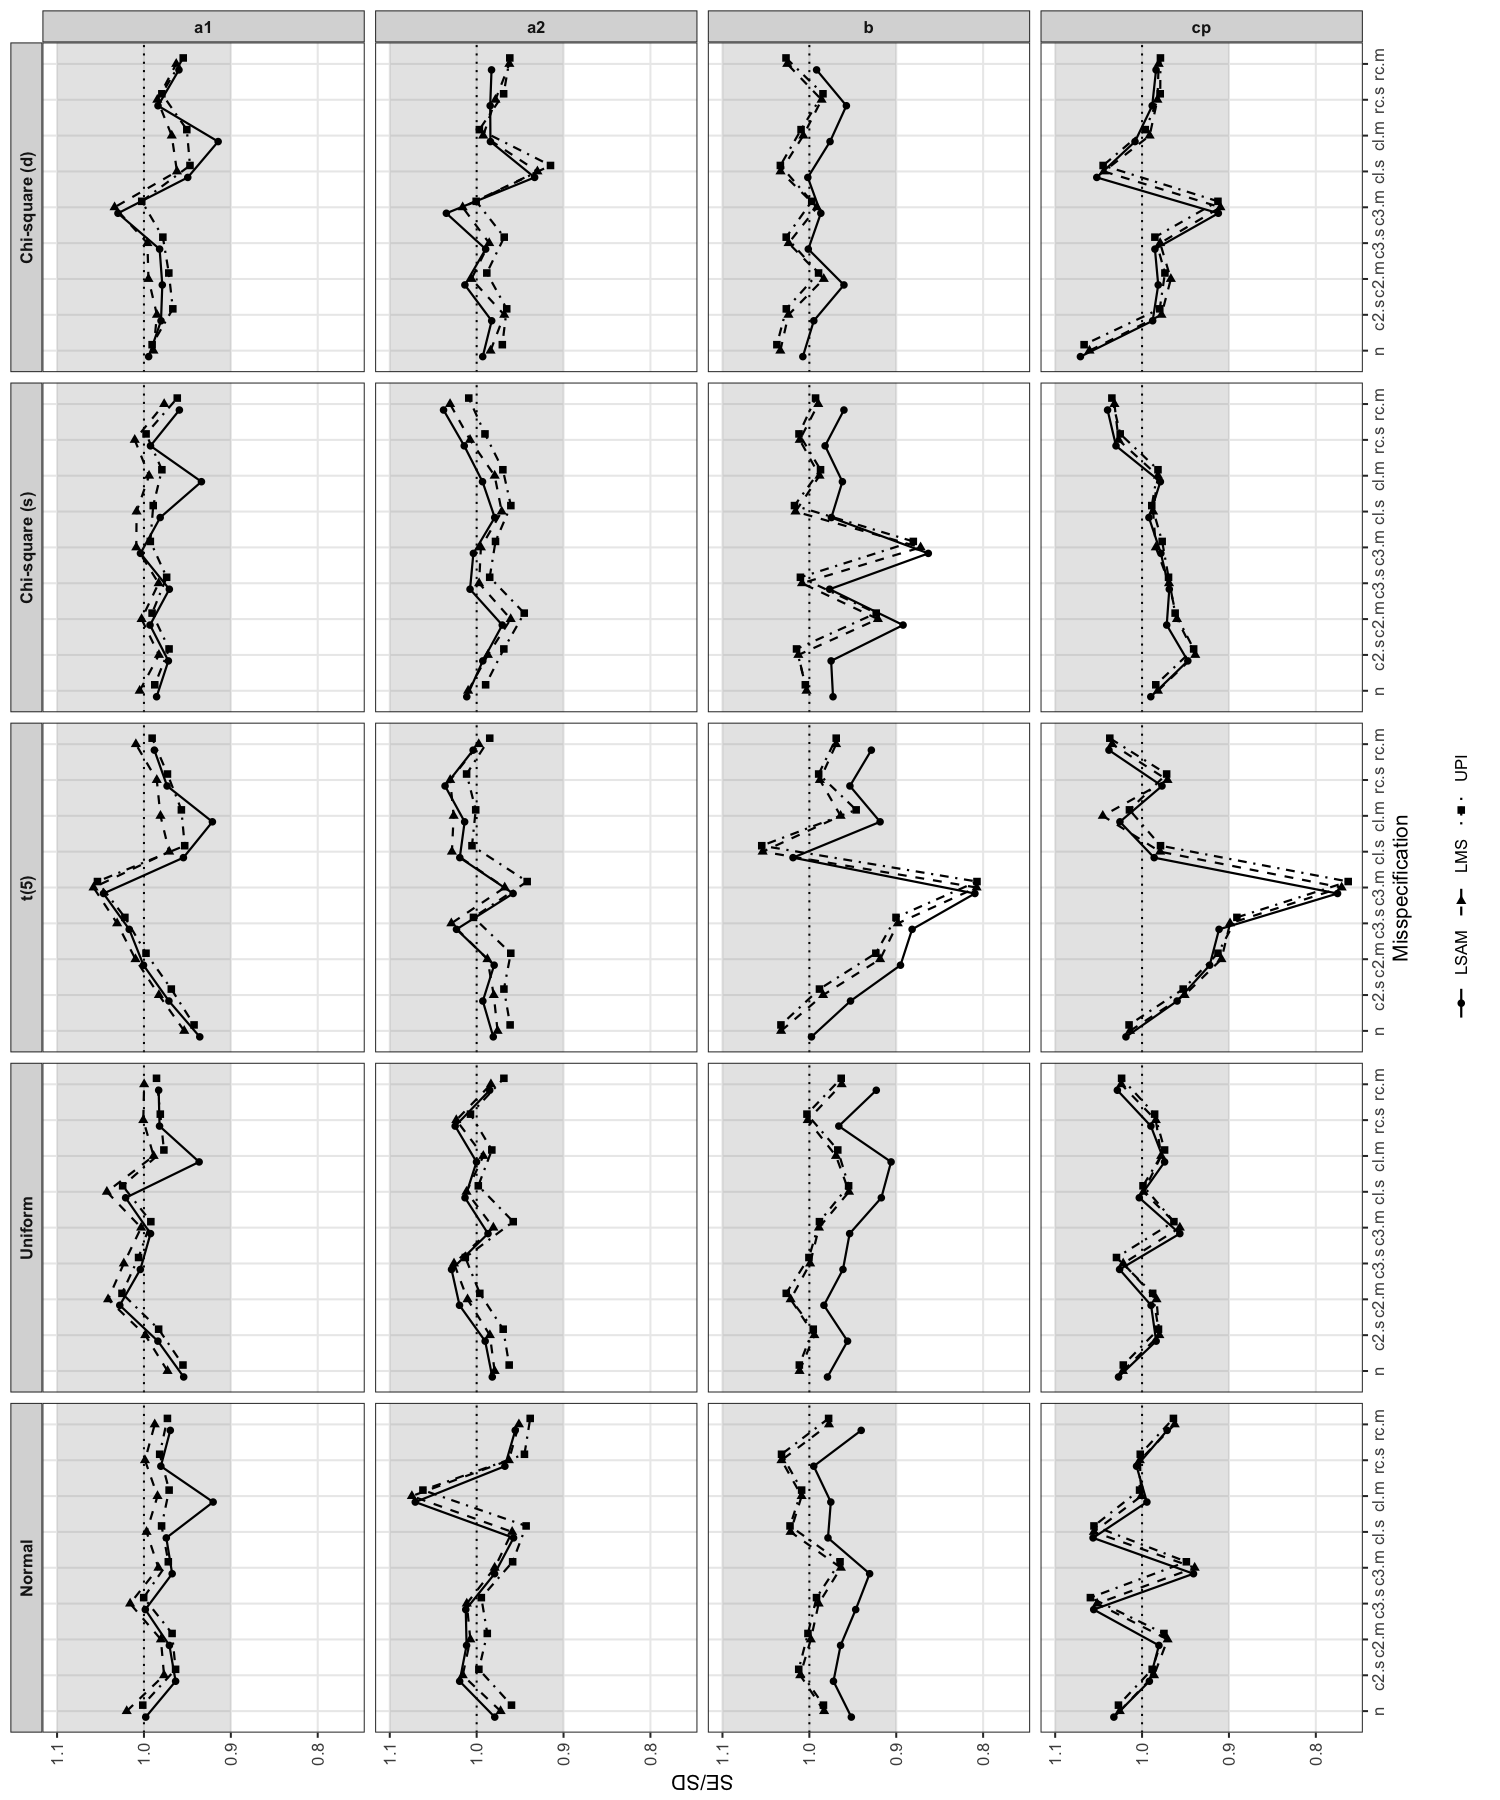
\includegraphics[width=6.3in,height=\textheight,keepaspectratio]{../plots/param_se_sd_a3-0.2_n500_high.png}

\vspace{-20pt}
\noindent \emph{Note.} The~gray band marks the acceptable region for the
measure. The Monte Carlo standard error (MCSE) is not computed for the
SE/SD ratio. LSAM = local structural-after-measurement; LMS = latent
moderated structural equations; UPI = unconstrained product indicator; n
= no misspecification.

\end{figure}

\subsection{Measurement Loadings}\label{measurement-loadings}

For the twelve freely estimated factor loadings, all but one are
recovered with acceptable performance across every measure and
essentially every condition, the exceptions being noisy deviations of
the relative bias of the variance estimator concentrated at \(N = 100\)
with low reliability. We display only the loading of the cross-loaded
mediator indicator \(m_3\), with its relative bias, coverage, SE/SD
ratio, and relative bias of the variance estimator at high reliability
and \(N = 500\) (Figure~\ref{fig-load}). For \(m_3\), \texttt{cl} is the
only consequential misspecification. Its relative bias rises sharply
under all approaches, less so under LSAM, and its coverage collapses
toward zero. The two standard error measures stay within the acceptable
range, except for LSAM under the medium \texttt{cl} with \(t_5\) and
\(\chi^2\) predictors. The remaining omissions leave the loading
unaffected.

\begin{figure}[!htbp]

{\caption{{Performance of the Cross-Loaded Mediator Indicator Loading
(\(m_3\)) Across All Measures, Distributions, and (Mis)specifications at
High Reliability, \(N = 500\), and \(a_3 = 0.2\)}{\label{fig-load}}}}

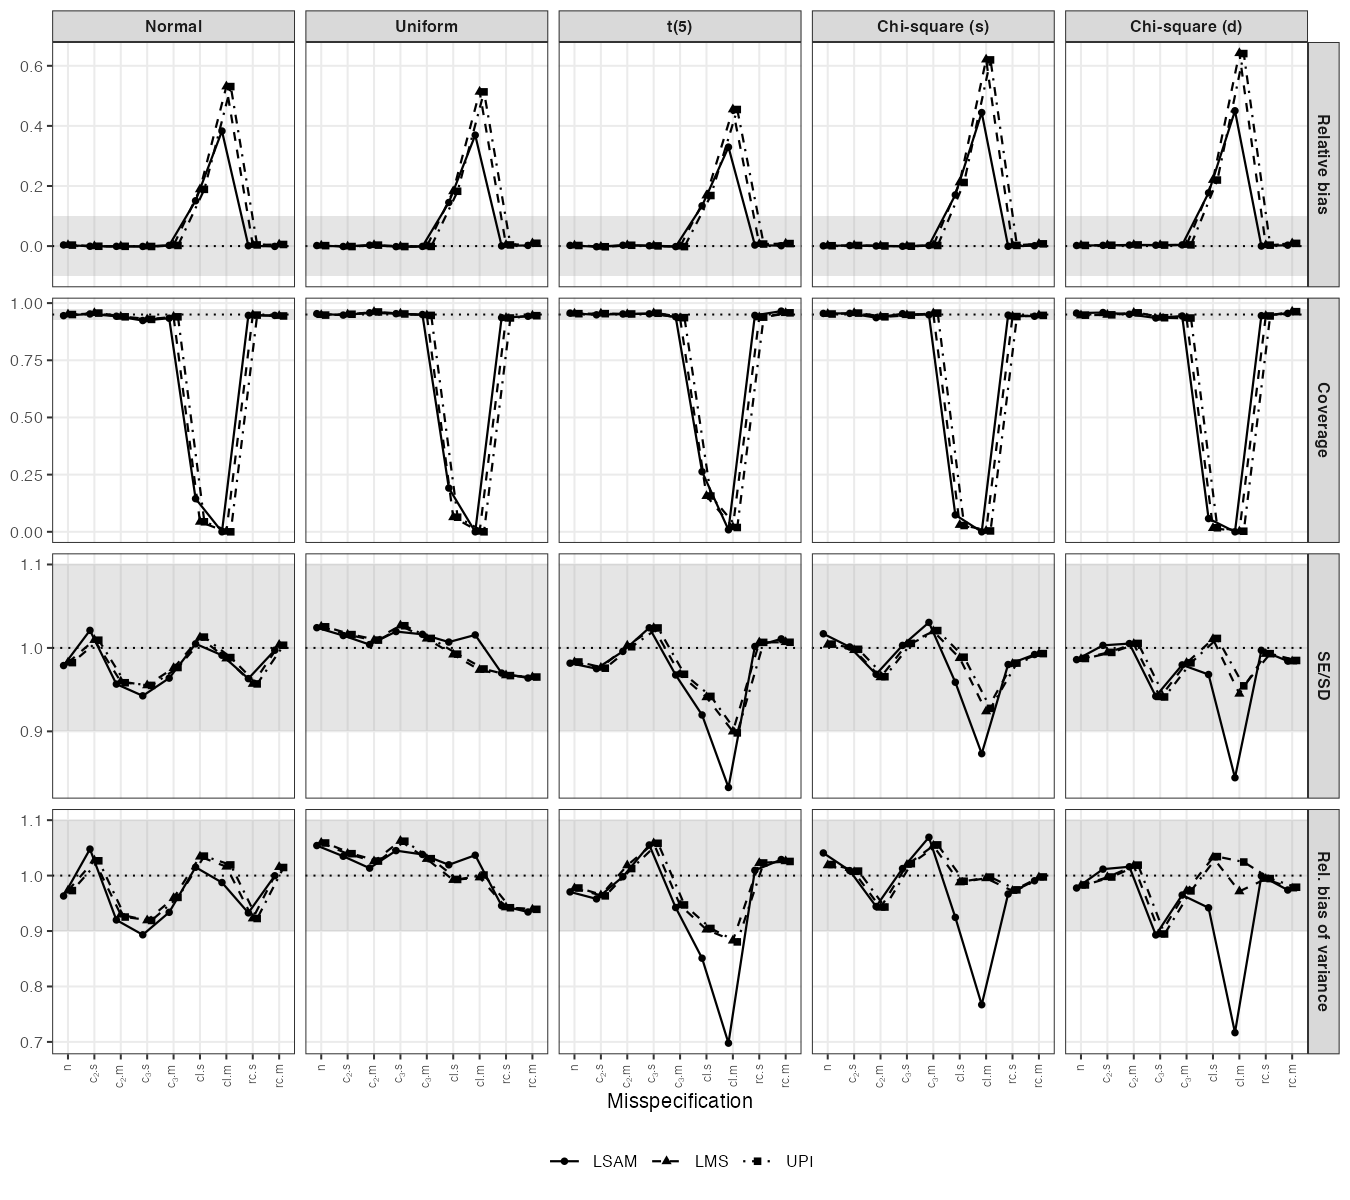
\includegraphics[width=1\linewidth,height=\textheight,keepaspectratio]{../plots/load_lm3_allmeasures_a3-0.2_n500_high.png}

\vspace{-20pt}
\noindent \emph{Note.} The~gray band in each panel marks the acceptable
region for that measure. LSAM = local structural-after-measurement; LMS
= latent moderated structural equations; UPI = unconstrained product
indicator; n = no misspecification.

\end{figure}

\section{Discussion}\label{discussion}

We evaluated three estimation approaches in the context of a latent
variable moderated mediation model, the two-step LSAM and the
system-wide LMS and UPI, under correct specification and under a large
number of structural and measurement misspecifications as well as
distributional violations.

Under correct specification with normal predictors, all three recovered
the imm and the interaction coefficient without bias and with nominal
coverage, differing mainly in the SE/SD ratio, Type I error, relative
RMSE, and power. LMS had the lowest relative RMSE and the highest power
but, under nonnormal predictors, showed bias under \(\chi^2\) predictors
at low reliability together with below-nominal coverage and inflated
Type I error. LSAM yielded Type I error closest to nominal, at the cost
of a higher relative RMSE and lower power in some cases, while UPI fell
in between, unbiased except at the smallest sample size with low
reliability, where it was also the least stable. Both standard error
measures stayed near one except in small samples, most at low
reliability, where UPI overestimated standard errors, and UPI and LSAM
struggled most under opposite-skewness \(\chi^2\) predictors.

Under misspecification, LSAM was the more robust approach. The
structural omissions in the outcome equation (\(c_2\), \(c_3\)) biased
the outcome-side coefficients for all approaches but left the mediator
equation, and hence the interaction coefficient, unaffected under LSAM,
whereas the system-wide approaches also carried them into the mediator
equation, biasing \(a_2\) under \(c_2\) and the interaction coefficient
under \(c_3\). The cross-loading (\texttt{cl}) was the most damaging
throughout. Under the system-wide approaches it biased the interaction
coefficient and most structural coefficients and sharply lowered
coverage at low reliability, while under LSAM it affected only \(a_1\)
and \(c'\) and left the coverage of the interaction coefficient near
nominal, although its standard errors for the affected loading were
underestimated under nonnormal predictors. The residual covariance
(\texttt{rc}) had little effect. Where bias was substantial, it was
smaller under LSAM, except for \(c'\) under the structural omissions,
where the three were similar, and it increased with the magnitude of the
omission and at lower reliability.

Regarding the imm, the Monte Carlo method delivered standard errors and
confidence intervals that behaved like those of the interaction
coefficient, with the deviations at low reliability and small samples
reflecting the standard errors of the underlying estimates. Under
misspecification its coverage dropped with the bias of its constituents
despite wider intervals. The method thus appears an adequate and far
cheaper alternative to the bootstrap here, although a direct comparison
remains to be made.

These patterns are broadly consistent with previous research. The
behavior of LMS and UPI under nonnormality and their stability under
normality reproduce earlier findings (Brandt et al., 2014; Cham et al.,
2012; Lonati et al., 2025; Vieira et al., 2026), as does that of LSAM
(Rosseel et al., 2025; Vieira et al., 2026). The measurement
misspecification results align with Brandt et al. (2020), where an
omitted cross-loading was likewise damaging for every estimator,
including UPI. Navarro and Schermelleh-Engel (2025) likewise found the
latent interaction effect underestimated under omitted cross-loadings
with LMS. Even so, Brandt et al. (2020) found no approach free of bias
and none uniformly best, as we also observed. Lastly, the contrast
between the structural and the measurement omissions matches the
expectation of Robitzsch (2022) that the advantage of SAM lies in
structural rather than measurement misspecification, since the
cross-loading biased LSAM as well, whereas the structural omissions left
its mediator equation untouched.

Finally, although we evaluated the estimation approaches from a
statistical perspective, the moderated mediation model itself rests on
strong causal assumptions (Imai et al., 2010; Rohrer et al., 2022). Good
statistical performance in certain conditions is therefore not, on its
own, a justification for a causal claim, and we direct interested
readers to the developing literature on the causal interpretation of
mediation (Imai et al., 2010; Morelli et al., 2026). Moreover,
misspecification had strong consequences across all three approaches,
and many of the omissions studied may be highly plausible in applied
contexts.

\newpage{}

\section{References}\label{references}

\protect\phantomsection\label{refs}
\begin{CSLReferences}{1}{0}
\bibitem[\citeproctext]{ref-BainterBollen2014}
Bainter, S. A., \& Bollen, K. A. (2014). Interpretational confounding or
confounded interpretations of causal indicators? \emph{Measurement:
Interdisciplinary Research and Perspectives}, \emph{12}(4), 125--140.
\url{https://doi.org/10.1080/15366367.2014.968503}

\bibitem[\citeproctext]{ref-Bohrnstedt1978}
Bohrnstedt, G. W., \& Marwell, G. (1978). The reliability of products of
two random variables. \emph{Sociological Methodology}, \emph{9},
254--273. \url{https://doi.org/10.2307/270812}

\bibitem[\citeproctext]{ref-Boker2023}
Boker, S. M., Oertzen, T. von, Pritikin, J. N., Hunter, M. D., Brick, T.
R., Brandmaier, A. M., \& Neale, M. C. (2023). Products of variables in
structural equation models. \emph{Structural Equation Modeling: A
Multidisciplinary Journal}, \emph{30}(5), 708--718.
\url{https://doi.org/10.1080/10705511.2022.2141749}

\bibitem[\citeproctext]{ref-Bollen1989}
Bollen, K. A. (1989). \emph{Structural equations with latent variables}.
John Wiley \& Sons. \url{https://doi.org/10.1002/9781118619179}

\bibitem[\citeproctext]{ref-Bollen1995}
Bollen, K. A. (1995). Structural equation models that are nonlinear in
latent variables: A least-squares estimator. \emph{Sociological
Methodology}, \emph{25}, 223--251. \url{https://doi.org/10.2307/271068}

\bibitem[\citeproctext]{ref-BollenHoyle2012}
Bollen, K. A., \& Hoyle, R. H. (2012). Latent variables in structural
equation modeling. In R. H. Hoyle (Ed.), \emph{Handbook of structural
equation modeling} (pp. 56--67). The Guilford Press.

\bibitem[\citeproctext]{ref-Brandt2014}
Brandt, H., Kelava, A., \& Klein, A. G. (2014). A simulation study
comparing recent approaches for the estimation of nonlinear effects in
{SEM} under the condition of nonnormality. \emph{Structural Equation
Modeling: A Multidisciplinary Journal}, \emph{21}(2), 181--195.
\url{https://doi.org/10.1080/10705511.2014.882660}

\bibitem[\citeproctext]{ref-Brandt2020}
Brandt, H., Umbach, N., Kelava, A., \& Bollen, K. A. (2020). Comparing
estimators for latent interaction models under structural and
distributional misspecifications. \emph{Psychological Methods},
\emph{25}(3), 321--345. \url{https://doi.org/10.1037/met0000231}

\bibitem[\citeproctext]{ref-Burt1976}
Burt, R. S. (1976). Interpretational confounding of unobserved variables
in structural equation models. \emph{Sociological Methods \& Research},
\emph{5}(1), 3--52. \url{https://doi.org/10.1177/004912417600500101}

\bibitem[\citeproctext]{ref-Busemeyer1983}
Busemeyer, J. R., \& Jones, L. E. (1983). Analysis of multiplicative
combination rules when the causal variables are measured with error.
\emph{Psychological Bulletin}, \emph{93}(3), 549--562.
\url{https://doi.org/10.1037/0033-2909.93.3.549}

\bibitem[\citeproctext]{ref-Cham2012}
Cham, H., West, S. G., Ma, Y., \& Aiken, L. S. (2012). Estimating latent
variable interactions with nonnormal observed data: A comparison of four
approaches. \emph{Multivariate Behavioral Research}, \emph{47}(6),
840--876. \url{https://doi.org/10.1080/00273171.2012.732901}

\bibitem[\citeproctext]{ref-Charlton2021}
Charlton, A., Montoya, A. K., Price, J., Hilgard, J., \&
Krefeld-Schwalb, A. (2021). \emph{Noise in the process: An assessment of
the evidential value of mediation effects in marketing journals}.
PsyArXiv preprint. \url{https://doi.org/10.31234/osf.io/ck2r5}

\bibitem[\citeproctext]{ref-CheungLau2008}
Cheung, G. W., \& Lau, R. S. (2008). Testing mediation and suppression
effects of latent variables: Bootstrapping with structural equation
models. \emph{Organizational Research Methods}, \emph{11}(2), 296--325.
\url{https://doi.org/10.1177/1094428107300343}

\bibitem[\citeproctext]{ref-CheungLau2017}
Cheung, G. W., \& Lau, R. S. (2017). Accuracy of parameter estimates and
confidence intervals in moderated mediation models: A comparison of
regression and latent moderated structural equations.
\emph{Organizational Research Methods}, \emph{20}(4), 746--769.
\url{https://doi.org/10.1177/1094428115595869}

\bibitem[\citeproctext]{ref-Cole2007}
Cole, D. A., Ciesla, J. A., \& Steiger, J. H. (2007). The insidious
effects of failing to include design-driven correlated residuals in
latent-variable covariance structure analysis. \emph{Psychological
Methods}, \emph{12}(4), 381--398.
\url{https://doi.org/10.1037/1082-989X.12.4.381}

\bibitem[\citeproctext]{ref-ColePreacher2014}
Cole, D. A., \& Preacher, K. J. (2014). Manifest variable path analysis:
Potentially serious and misleading consequences due to uncorrected
measurement error. \emph{Psychological Methods}, \emph{19}(2), 300--315.
\url{https://doi.org/10.1037/a0033805}

\bibitem[\citeproctext]{ref-CoxKelcey2021}
Cox, K., \& Kelcey, B. (2021). {Croon}'s bias-corrected estimation of
latent interactions. \emph{Structural Equation Modeling: A
Multidisciplinary Journal}, \emph{28}(6), 863--874.
\url{https://doi.org/10.1080/10705511.2021.1922283}

\bibitem[\citeproctext]{ref-DeShon1998}
DeShon, R. P. (1998). A cautionary note on measurement error corrections
in structural equation models. \emph{Psychological Methods},
\emph{3}(4), 412--423. \url{https://doi.org/10.1037/1082-989X.3.4.412}

\bibitem[\citeproctext]{ref-dolstra_etall_2004}
Dolstra, E., De Jonge, M., \& Visser, E. (2004). {Nix}: A safe and
policy-free system for software deployment. \emph{18th Large
Installation System Administration Conference}, 79--92.

\bibitem[\citeproctext]{ref-Edwards2007}
Edwards, J. R., \& Lambert, L. S. (2007). Methods for integrating
moderation and mediation: A general analytical framework using moderated
path analysis. \emph{Psychological Methods}, \emph{12}(1), 1--22.
\url{https://doi.org/10.1037/1082-989X.12.1.1}

\bibitem[\citeproctext]{ref-FalkBiesanz2015}
Falk, C. F., \& Biesanz, J. C. (2015). Inference and interval estimation
methods for indirect effects with latent variable models.
\emph{Structural Equation Modeling: A Multidisciplinary Journal},
\emph{22}(1), 24--38. \url{https://doi.org/10.1080/10705511.2014.935266}

\bibitem[\citeproctext]{ref-Feng2020}
Feng, Q., Song, Q., Zhang, L., Zheng, S., \& Pan, J. (2020). Integration
of moderation and mediation in a latent variable framework: A comparison
of estimation approaches for the second-stage moderated mediation model.
\emph{Frontiers in Psychology}, \emph{11}, 2167.
\url{https://doi.org/10.3389/fpsyg.2020.02167}

\bibitem[\citeproctext]{ref-Fritz2016}
Fritz, M. S., Kenny, D. A., \& MacKinnon, D. P. (2016). The combined
effects of measurement error and omitting confounders in the
single-mediator model. \emph{Multivariate Behavioral Research},
\emph{51}(5), 681--697.
\url{https://doi.org/10.1080/00273171.2016.1224154}

\bibitem[\citeproctext]{ref-GonzalezMacKinnon2021}
Gonzalez, O., \& MacKinnon, D. P. (2021). The measurement of the
mediator and its influence on statistical mediation conclusions.
\emph{Psychological Methods}, \emph{26}(1), 1--17.
\url{https://doi.org/10.1037/met0000263}

\bibitem[\citeproctext]{ref-Gronneberg2022}
Grønneberg, S., Foldnes, N., \& Marcoulides, K. M. (2022). {covsim}: An
{R} package for simulating non-normal data for structural equation
models using copulas. \emph{Journal of Statistical Software},
\emph{102}(3), 1--45. \url{https://doi.org/10.18637/jss.v102.i03}

\bibitem[\citeproctext]{ref-Hayes2015}
Hayes, A. F. (2015). An index and test of linear moderated mediation.
\emph{Multivariate Behavioral Research}, \emph{50}(1), 1--22.
\url{https://doi.org/10.1080/00273171.2014.962683}

\bibitem[\citeproctext]{ref-Hayes2018}
Hayes, A. F. (2018). \emph{Introduction to mediation, moderation, and
conditional process analysis: A regression-based approach} (2nd ed.).
The Guilford Press.

\bibitem[\citeproctext]{ref-HolstBudtz2020}
Holst, K. K., \& Budtz-Jørgensen, E. (2020). A two-stage estimation
procedure for non-linear structural equation models.
\emph{Biostatistics}, \emph{21}(4), 676--691.
\url{https://doi.org/10.1093/biostatistics/kxy082}

\bibitem[\citeproctext]{ref-HoyleKenny1999}
Hoyle, R. H., \& Kenny, D. A. (1999). Sample size, reliability, and
tests of statistical mediation. In R. H. Hoyle (Ed.), \emph{Statistical
strategies for small sample research} (pp. 195--222). Sage.

\bibitem[\citeproctext]{ref-Imai2010}
Imai, K., Keele, L., \& Tingley, D. (2010). A general approach to causal
mediation analysis. \emph{Psychological Methods}, \emph{15}(4),
309--334. \url{https://doi.org/10.1037/a0020761}

\bibitem[\citeproctext]{ref-Joshi2025}
Joshi, M., \& Pustejovsky, J. (2025). \emph{{simhelpers}: Helper
functions for simulation studies}.
\url{https://CRAN.R-project.org/package=simhelpers}

\bibitem[\citeproctext]{ref-KelavaBrandt2009}
Kelava, A., \& Brandt, H. (2009). Estimation of nonlinear latent
structural equation models using the extended unconstrained approach.
\emph{Review of Psychology}, \emph{16}(2), 123--131.

\bibitem[\citeproctext]{ref-KelavaBrandt2022}
Kelava, A., \& Brandt, H. (2022). Latent interaction effects. In R. H.
Hoyle (Ed.), \emph{Handbook of structural equation modeling} (pp.
427--446). Guilford Press.

\bibitem[\citeproctext]{ref-Kelava2011}
Kelava, A., Werner, C. S., Schermelleh-Engel, K., Moosbrugger, H., Zapf,
D., Ma, Y., Cham, H., Aiken, L. S., \& West, S. G. (2011). Advanced
nonlinear latent variable modeling: Distribution analytic {LMS} and
{QML} estimators of interaction and quadratic effects. \emph{Structural
Equation Modeling: A Multidisciplinary Journal}, \emph{18}(3), 465--491.
\url{https://doi.org/10.1080/10705511.2011.582408}

\bibitem[\citeproctext]{ref-Keller2025}
Keller, B. T. (2025). A factored regression approach to modeling latent
variable interactions and nonlinear effects. \emph{Psychological
Methods}. \url{https://doi.org/10.1037/met0000777}

\bibitem[\citeproctext]{ref-KennyJudd1984}
Kenny, D. A., \& Judd, C. M. (1984). Estimating the nonlinear and
interactive effects of latent variables. \emph{Psychological Bulletin},
\emph{96}(1), 201--210. \url{https://doi.org/10.1037/0033-2909.96.1.201}

\bibitem[\citeproctext]{ref-KleinMoosbrugger2000}
Klein, A. G., \& Moosbrugger, H. (2000). Maximum likelihood estimation
of latent interaction effects with the {LMS} method.
\emph{Psychometrika}, \emph{65}(4), 457--474.
\url{https://doi.org/10.1007/BF02296338}

\bibitem[\citeproctext]{ref-KleinMuthen2007}
Klein, A. G., \& Muthén, B. O. (2007). Quasi-maximum likelihood
estimation of structural equation models with multiple interaction and
quadratic effects. \emph{Multivariate Behavioral Research},
\emph{42}(4), 647--673. \url{https://doi.org/10.1080/00273170701710205}

\bibitem[\citeproctext]{ref-LedgerwoodShrout2011}
Ledgerwood, A., \& Shrout, P. E. (2011). The trade-off between accuracy
and precision in latent variable models of mediation processes.
\emph{Journal of Personality and Social Psychology}, \emph{101}(6),
1174--1188. \url{https://doi.org/10.1037/a0024776}

\bibitem[\citeproctext]{ref-Lin2010}
Lin, G.-C., Wen, Z., Marsh, H. W., \& Lin, H.-S. (2010). Structural
equation models of latent interactions: Clarification of orthogonalizing
and double-mean-centering strategies. \emph{Structural Equation
Modeling: A Multidisciplinary Journal}, \emph{17}(3), 374--391.
\url{https://doi.org/10.1080/10705511.2010.488999}

\bibitem[\citeproctext]{ref-Lonati2025}
Lonati, S., Rönkkö, M., \& Antonakis, J. (2025). Normality assumption in
latent interaction models. \emph{Psychological Methods}, \emph{30}(6),
1242--1262. \url{https://doi.org/10.1037/met0000657}

\bibitem[\citeproctext]{ref-MacKinnonFairchild2007}
MacKinnon, D. P., Fairchild, A. J., \& Fritz, M. S. (2007). Mediation
analysis. \emph{Annual Review of Psychology}, \emph{58}, 593--614.
\url{https://doi.org/10.1146/annurev.psych.58.110405.085542}

\bibitem[\citeproctext]{ref-MacKinnonLockwood2004}
MacKinnon, D. P., Lockwood, C. M., \& Williams, J. (2004). Confidence
limits for the indirect effect: Distribution of the product and
resampling methods. \emph{Multivariate Behavioral Research},
\emph{39}(1), 99--128. \url{https://doi.org/10.1207/s15327906mbr3901_4}

\bibitem[\citeproctext]{ref-Marsh2004}
Marsh, H. W., Wen, Z., \& Hau, K.-T. (2004). Structural equation models
of latent interactions: Evaluation of alternative estimation strategies
and indicator construction. \emph{Psychological Methods}, \emph{9}(3),
275--300. \url{https://doi.org/10.1037/1082-989X.9.3.275}

\bibitem[\citeproctext]{ref-McNeishWolf2020}
McNeish, D., \& Wolf, M. G. (2020). Thinking twice about sum scores.
\emph{Behavior Research Methods}, \emph{52}(6), 2287--2305.
\url{https://doi.org/10.3758/s13428-020-01398-0}

\bibitem[\citeproctext]{ref-Montoya2024}
Montoya, A. K. (2024). Combining statistical and causal mediation
analysis. In H. T. Reis, T. West, \& C. M. Judd (Eds.), \emph{Handbook
of research methods in social and personality psychology} (pp.
622--652). Cambridge University Press.

\bibitem[\citeproctext]{ref-MooijaartBentler2010}
Mooijaart, A., \& Bentler, P. M. (2010). An alternative approach for
nonlinear latent variable models. \emph{Structural Equation Modeling: A
Multidisciplinary Journal}, \emph{17}(3), 357--373.
\url{https://doi.org/10.1080/10705511.2010.488997}

\bibitem[\citeproctext]{ref-Morelli2026}
Morelli, S., Faleh, R., \& Brandt, H. (2026). \emph{{RAPSEM}:
Identifying latent mediators without sequential ignorability via a
rank-preserving structural equation model}. arXiv preprint
arXiv:2509.23935. \url{https://doi.org/10.48550/arXiv.2509.23935}

\bibitem[\citeproctext]{ref-Nagler2025}
Nagler, T., \& Vatter, T. (2025). \emph{{rvinecopulib}: High performance
algorithms for vine copula modeling}.
\url{https://CRAN.R-project.org/package=rvinecopulib}

\bibitem[\citeproctext]{ref-NavarroSchermelleh2025}
Navarro, K., \& Schermelleh-Engel, K. (2025). Cause for concern: Omitted
cross-loadings in measurement models of nonlinear structural equation
models. \emph{Behavior Research Methods}, \emph{57}(328).
\url{https://doi.org/10.3758/s13428-025-02792-2}

\bibitem[\citeproctext]{ref-NgChan2020}
Ng, J. C. K., \& Chan, W. (2020). Latent moderation analysis: A factor
score approach. \emph{Structural Equation Modeling: A Multidisciplinary
Journal}, \emph{27}(4), 629--648.
\url{https://doi.org/10.1080/10705511.2019.1664304}

\bibitem[\citeproctext]{ref-Pawel2026}
Pawel, S., Bartoš, F., Siepe, B. S., \& Lohmann, A. (2026). Handling
missingness, failures, and non-convergence in simulation studies: A
review of current practices and recommendations. \emph{The American
Statistician}, \emph{80}(1), 31--48.
\url{https://doi.org/10.1080/00031305.2025.2540002}

\bibitem[\citeproctext]{ref-Pieters2017}
Pieters, R. (2017). Meaningful mediation analysis: Plausible causal
inference and informative communication. \emph{Journal of Consumer
Research}, \emph{44}(3), 692--716.
\url{https://doi.org/10.1093/jcr/ucx081}

\bibitem[\citeproctext]{ref-Preacher2007}
Preacher, K. J., Rucker, D. D., \& Hayes, A. F. (2007). Addressing
moderated mediation hypotheses: Theory, methods, and prescriptions.
\emph{Multivariate Behavioral Research}, \emph{42}(1), 185--227.
\url{https://doi.org/10.1080/00273170701341316}

\bibitem[\citeproctext]{ref-PreacherSelig2012}
Preacher, K. J., \& Selig, J. P. (2012). Advantages of monte carlo
confidence intervals for indirect effects. \emph{Communication Methods
and Measures}, \emph{6}(2), 77--98.
\url{https://doi.org/10.1080/19312458.2012.679848}

\bibitem[\citeproctext]{ref-RCoreTeam}
R Core Team. (2025). \emph{R: A language and environment for statistical
computing}. R Foundation for Statistical Computing.
\url{https://www.R-project.org/}

\bibitem[\citeproctext]{ref-Rhemtulla2020}
Rhemtulla, M., Bork, R. van, \& Borsboom, D. (2020). Worse than
measurement error: Consequences of inappropriate latent variable
measurement models. \emph{Psychological Methods}, \emph{25}(1), 30--45.
\url{https://doi.org/10.1037/met0000220}

\bibitem[\citeproctext]{ref-Rimpler2026}
Rimpler, A., Kiers, H. A. L., \& Ravenzwaaij, D. van. (2026). Anything
goes: Statistical interactions without substantive theory.
\emph{Computational Brain \& Behavior}.
\url{https://doi.org/10.1007/s42113-026-00305-8}

\bibitem[\citeproctext]{ref-Robitzsch2022}
Robitzsch, A. (2022). Comparing the robustness of the structural after
measurement ({SAM}) approach to structural equation modeling ({SEM})
against local model misspecifications with alternative estimation
approaches. \emph{Stats}, \emph{5}(3), 631--672.
\url{https://doi.org/10.3390/stats5030039}

\bibitem[\citeproctext]{ref-rix}
Rodrigues, B., \& Baumann, P. (2026). \emph{Rix: Reproducible data
science environments with {Nix}}.
\url{https://CRAN.R-project.org/package=rix}

\bibitem[\citeproctext]{ref-Rohrer2022}
Rohrer, J. M., Hünermund, P., Arslan, R. C., \& Elson, M. (2022). That's
a lot to process! Pitfalls of popular path models. \emph{Advances in
Methods and Practices in Psychological Science}, \emph{5}(2), 1--14.
\url{https://doi.org/10.1177/25152459221095827}

\bibitem[\citeproctext]{ref-Rosseel2012}
Rosseel, Y. (2012). {lavaan}: An {R} package for structural equation
modeling. \emph{Journal of Statistical Software}, \emph{48}(2), 1--36.
\url{https://doi.org/10.18637/jss.v048.i02}

\bibitem[\citeproctext]{ref-Rosseel2025}
Rosseel, Y., Burghgraeve, E., Loh, W. W., \& Schermelleh-Engel, K.
(2025). Structural after measurement ({SAM}) approaches for
accommodating latent quadratic and interaction effects. \emph{Behavior
Research Methods}, \emph{57}(4), 101.
\url{https://doi.org/10.3758/s13428-024-02532-y}

\bibitem[\citeproctext]{ref-RosseelLoh2024}
Rosseel, Y., \& Loh, W. W. (2024). A structural after measurement
approach to structural equation modeling. \emph{Psychological Methods},
\emph{29}(3), 561--588. \url{https://doi.org/10.1037/met0000503}

\bibitem[\citeproctext]{ref-apaquarto}
Schneider, W. J. (2026). \emph{{apaquarto}: A {Quarto} extension for
creating {APA} style ({7th} edition) documents}.
\url{https://github.com/wjschne/apaquarto}

\bibitem[\citeproctext]{ref-Siepe2024}
Siepe, B. S., Bartoš, F., Morris, T. P., Boulesteix, A.-L., Heck, D. W.,
\& Pawel, S. (2024). Simulation studies for methodological research in
psychology: A standardized template for planning, preregistration, and
reporting. \emph{Psychological Methods}.
\url{https://doi.org/10.1037/met0000695}

\bibitem[\citeproctext]{ref-Slupphaug2025}
Slupphaug, K. S., Mehmetoglu, M., \& Mittner, M. (2025). {modsem}: An
{R} package for estimating latent interactions and quadratic effects.
\emph{Structural Equation Modeling: A Multidisciplinary Journal},
\emph{32}(4), 717--729.
\url{https://doi.org/10.1080/10705511.2024.2417409}

\bibitem[\citeproctext]{ref-Sterner2024}
Sterner, P., Pargent, F., Deffner, D., \& Goretzko, D. (2024). A causal
framework for the comparability of latent variables. \emph{Structural
Equation Modeling: A Multidisciplinary Journal}, \emph{31}(5), 747--758.
\url{https://doi.org/10.1080/10705511.2024.2339396}

\bibitem[\citeproctext]{ref-Tibbe2022}
Tibbe, T. D., \& Montoya, A. K. (2022). Correcting the bias correction
for the bootstrap confidence interval in mediation analysis.
\emph{Frontiers in Psychology}, \emph{13}, 810258.
\url{https://doi.org/10.3389/fpsyg.2022.810258}

\bibitem[\citeproctext]{ref-VanderWeele2009}
VanderWeele, T. J. (2009). On the distinction between interaction and
effect modification. \emph{Epidemiology}, \emph{20}(6), 863--871.
\url{https://doi.org/10.1097/EDE.0b013e3181ba333c}

\bibitem[\citeproctext]{ref-VanderWeeleValeri2012}
VanderWeele, T. J., Valeri, L., \& Ogburn, E. L. (2012). The role of
measurement error and misclassification in mediation analysis.
\emph{Epidemiology}, \emph{23}(4), 561--564.
\url{https://doi.org/10.1097/EDE.0b013e318258f5e4}

\bibitem[\citeproctext]{ref-VanderWeeleVansteelandt2022}
VanderWeele, T. J., \& Vansteelandt, S. (2022). A statistical test to
reject the structural interpretation of a latent factor model.
\emph{Journal of the Royal Statistical Society: Series B (Statistical
Methodology)}, \emph{84}(5), 2032--2054.
\url{https://doi.org/10.1111/rssb.12555}

\bibitem[\citeproctext]{ref-Vieira2026}
Vieira, F. F., Slupphaug, K. S., \& Rosseel, Y. (2026). Evaluating local
structural-after-measurement and traditional approaches for the
estimation of complex nonlinear effects among latent variables.
\emph{Psychological Methods}. \url{https://doi.org/10.1037/met0000851}

\bibitem[\citeproctext]{ref-WallAmemiya2000}
Wall, M. M., \& Amemiya, Y. (2000). Estimation for polynomial structural
equation models. \emph{Journal of the American Statistical Association},
\emph{95}(451), 929--940. \url{https://doi.org/10.2307/2669475}

\bibitem[\citeproctext]{ref-WallAmemiya2003}
Wall, M. M., \& Amemiya, Y. (2003). A method of moments technique for
fitting interaction effects in structural equation models. \emph{British
Journal of Mathematical and Statistical Psychology}, \emph{56}(1),
47--63. \url{https://doi.org/10.1348/000711003321645331}

\bibitem[\citeproctext]{ref-WangRhemtulla2021}
Wang, Y. A., \& Rhemtulla, M. (2021). Power analysis for parameter
estimation in structural equation modeling: A discussion and tutorial.
\emph{Advances in Methods and Practices in Psychological Science},
\emph{4}(1), 1--17. \url{https://doi.org/10.1177/2515245920918253}

\end{CSLReferences}

\newpage{}

\appendix

\section{Calibration and Data Generation}\label{apx-calibration}

This appendix gives the formulas behind the data-generating mechanism.
The calibration that fixes the variance parameters comes first, followed
by the three-stage data generation that uses them.

\subsection{Calibration}\label{calibration}

The structural disturbance variances and indicator error variances were
fixed by the following closed-form calibration, computed once under the
normal baseline.

\subsubsection{Structural residual
variances}\label{structural-residual-variances}

The disturbance variances \(\psi_M, \psi_Y\) are fixed so that each
structural equation explains a fraction \(R^2 \approx 0.30\) of its
outcome's variance at the central interaction level \(a_3 = 0.2\) under
the normal baseline. Writing the systematic part of \(M\) as
\(S_M = a_1 X + a_2 W + a_3 (X W)\), its variance needs only second
moments,

\[
\operatorname{Var}(S_M) = a_1^2 + a_2^2 + 2 a_1 a_2 \rho + a_3^2 (1 + \rho^2),
\]

\noindent and the disturbance is the remainder that brings the signal
share to \(R^2\),

\[
\psi_M = \operatorname{Var}(S_M)\,\frac{1 - R^2}{R^2}, \qquad
\psi_Y = \operatorname{Var}(b M + c' X)\,\frac{1 - R^2}{R^2},
\]

\noindent with
\(\operatorname{Var}(b M + c' X) = b^2 \operatorname{Var}(M) + c'^2 + 2 b c'\,(a_1 + a_2 \rho)\).
Fixed at these values, the population variances of \(M\) and \(Y\) are
closed-form functions of the parameters,

\[
\operatorname{Var}(M) = \operatorname{Var}(S_M) + \psi_M, \qquad
\operatorname{Var}(Y) = b^2 \operatorname{Var}(M) + c'^2 + 2 b c'\,(a_1 + a_2 \rho) + \psi_Y,
\]

\noindent evaluated once under the normal baseline and held fixed across
distributions, so that \(R^2\) and reliability drift only through the
design factors.

\subsubsection{Indicator reliabilities}\label{indicator-reliabilities}

To hit a target reliability \(\omega \in \{0.5, 0.7\}\), the error
variance of indicator \(j\) is set from the latent variance
\(V = \operatorname{Var}(\eta)\),

\[
\theta_{\eta j} = \lambda_j^2\, V\,\frac{1 - \omega}{\omega}.
\]

For \(X, W\) the variance is exactly \(1\); for \(M, Y\) it is the
closed form above, fixed at the normal baseline, so the realized
reliability drifts mildly across distributions.

\subsubsection{Calibrating the misspecification
magnitudes}\label{calibrating-the-misspecification-magnitudes}

The \emph{small} and \emph{medium} labels are standardized coefficients,
\(t \in \{0.25, 0.50\}\). For an omitted predictor \(p\) added to a
baseline outcome \(y_0\), the magnitude is the fully standardized
regression coefficient of \(p\),

\[
t = \frac{\beta\,\operatorname{sd}(p)}{\operatorname{sd}(y_0 + \beta p)}.
\]

Squaring and substituting
\(\operatorname{Var}(y_0 + \beta p) = \operatorname{Var}(y_0) + \beta^2 \operatorname{Var}(p) + 2 \beta \operatorname{Cov}(p, y_0)\)
yields a quadratic \(A\beta^2 + B\beta + C = 0\) with

\[
A = \operatorname{Var}(p)\,(1 - t^2), \quad
B = -2 t^2 \operatorname{Cov}(p, y_0), \quad
C = -t^2 \operatorname{Var}(y_0).
\]

Since \(A > 0\) and \(C < 0\) the roots have opposite sign; the positive
omitted path is the positive root,

\[
\beta = \frac{t^2 \operatorname{Cov}(p, y_0) + \sqrt{\,t^4 \operatorname{Cov}(p, y_0)^2 + t^2 (1 - t^2)\,\operatorname{Var}(p)\,\operatorname{Var}(y_0)\,}}{\operatorname{Var}(p)\,(1 - t^2)}.
\]

The three moments are estimated from one large (\(n = 10^6\)) sample per
distribution and \(a_3\) level. The predictor \(p\) and baseline \(y_0\)
differ by misspecification,

\[
\begin{aligned}
c_2: \quad & p = W,   && y_0 = b M + c' X + \zeta_Y, \\
c_3: \quad & p = X W, && y_0 = b M + c' X + \zeta_Y, \\
\texttt{cl}: \quad & p = X,   && y_0 = m_3 = \lambda_3 M + \delta_{m_3}.
\end{aligned}
\]

\(c_2\) and \(c_3\) are reliability independent; \texttt{cl} depends on
\(\omega\) because its baseline \(m_3\) carries measurement noise.
\texttt{rc} never enters the calibration: it is a residual correlation
and equals its target in every cell.

\subsubsection{\texorpdfstring{Holding \(Y\) reliability fixed under
\(c_2\) and
\(c_3\)}{Holding Y reliability fixed under c\_2 and c\_3}}\label{holding-y-reliability-fixed-under-c_2-and-c_3}

Adding an omitted structural path inflates \(\operatorname{Var}(Y)\) by
\(\kappa = \operatorname{Var}(y_0 + \beta p) / \operatorname{Var}(y_0)\),
which would raise \(Y\)'s indicator reliability as a side effect.
Scaling the \(Y\)-indicator noise by the same \(\kappa\) makes signal
and noise move together, so \(\kappa\) cancels and the reliability
returns to its no-misspecification value,

\[
\omega_j = \frac{\kappa\,\lambda_j^2 V}{\kappa\,\lambda_j^2 V + \kappa\,\theta_j}
= \frac{\lambda_j^2 V}{\lambda_j^2 V + \theta_j}.
\]

The latent effect size is untouched; only the \(Y\) indicators are made
correspondingly noisier. The measurement level misspecifications
\texttt{cl} and \texttt{rc} act on the indicators directly and are not
compensated, since that contamination is itself the misspecification.

\subsection{Data generation}\label{data-generation-1}

Using the calibrated variances above, data were generated in three
stages: the correlated exogenous predictors, the dependent latent
variables through the structural model, and the observed indicators
through the measurement model.

\subsubsection{Stage I: Exogenous
predictors}\label{stage-i-exogenous-predictors}

The correlated predictors \((X, W)\) were generated with the
vine-to-anything (VITA) method (Grønneberg et al., 2022), as implemented
in the \emph{covsim} package, with sampling via \emph{rvinecopulib}
(Nagler \& Vatter, 2025). They were specified to have mean \(0\),
variance \(1\), and the covariance structure

\[
\Phi = \begin{bmatrix} 1 & \rho \\ \rho & 1 \end{bmatrix}
     = \begin{bmatrix} 1 & 0.3 \\ 0.3 & 1 \end{bmatrix},
\]

\noindent so that the conditions differ only in distributional shape.
Under the normal condition, the predictors had Gaussian marginals with
the specified covariance structure. Under the uniform condition, they
had symmetric uniform marginals \(\mathrm{U}(-\sqrt3, \sqrt3)\), which
have mean \(0\) and variance \(1\). Under the \(t_5\) condition, they
had Student \(t\) marginals with five degrees of freedom, rescaled by
\(\sqrt{5/3}\) to unit variance. The two \(\chi^2\) conditions used
\(\chi^2_2\) marginals, centered by their mean (\(2\)) and scaled by
their standard deviation (\(2\)) to mean \(0\) and variance \(1\). In
the same-direction condition both predictors are right-skewed, whereas
in the opposite-direction condition \(W\) is negated so that \(X\) and
\(W\) are skewed in opposite directions, with the sampled correlation
sign flipped to restore \(\operatorname{Cor}(X, W) = \rho\). In every
condition, VITA constructed a vine copula to impose \(\Phi\) while
preserving the marginals.

\subsubsection{Stage II: Structural
model}\label{stage-ii-structural-model}

The dependent latent variables were generated from the structural
equations

\[
M = a_1 X + a_2 W + a_3 (X \times W) + \zeta_M, \qquad
Y = b M + c' X + \zeta_Y,
\]

\noindent with independent Gaussian disturbances
\(\zeta_M \sim \mathcal{N}(0, \psi_M)\) and
\(\zeta_Y \sim \mathcal{N}(0, \psi_Y)\). The disturbance variances
\(\psi_M, \psi_Y\) take the calibrated values so that each equation
explains \(R^2 \approx 0.30\) of its outcome's variance at the central
interaction level under the normal baseline.

\subsubsection{Stage III: Measurement
model}\label{stage-iii-measurement-model}

Each latent \(\eta \in \{X, W, M, Y\}\) was measured by four indicators,

\[
z_{\eta j} = \lambda_j\,\eta + \delta_{\eta j}, \qquad \lambda = (1, 0.8, 0.7, 0.6),
\]

\noindent with independent Gaussian errors
\(\delta_{\eta j} \sim \mathcal{N}(0, \theta_{\eta j})\). The error
variances \(\theta_{\eta j}\) take the calibrated values that achieve
the target reliability \(\omega \in \{0.5, 0.7\}\). Only the exogenous
predictors varied in distribution. The structural disturbances and
measurement errors were Gaussian in every condition.






\end{document}
